%%%%%%%%%%%%%%%%%%%%%%%%%%%%%%%%%%%%%%%%%%%%%%%%%%%%%%%%%%%%
%  Axiomatizing AI: Emergence Under Scaling
%  Author: Isidor Manning
%  Clean & Structured LaTeX Header (2025)
%%%%%%%%%%%%%%%%%%%%%%%%%%%%%%%%%%%%%%%%%%%%%%%%%%%%%%%%%%%%

\documentclass[12pt]{article}

%%%%%%%%%%%%%%%%%%%%%%%%%%%%%%%%%%%%%%%%%%%%%%%%%%%%%%%%%%%%
% --- PAGE GEOMETRY & LAYOUT ---
%%%%%%%%%%%%%%%%%%%%%%%%%%%%%%%%%%%%%%%%%%%%%%%%%%%%%%%%%%%%
\usepackage[
  margin=1.5in,
  includefoot
]{geometry}

\usepackage{setspace}        % Line spacing control
\usepackage{parskip}         % No paragraph indentation, vertical space between paragraphs
\setlength{\parindent}{0pt}
\setlength{\parskip}{6pt}

%%%%%%%%%%%%%%%%%%%%%%%%%%%%%%%%%%%%%%%%%%%%%%%%%%%%%%%%%%%%
% --- TYPOGRAPHY & READABILITY ---
%%%%%%%%%%%%%%%%%%%%%%%%%%%%%%%%%%%%%%%%%%%%%%%%%%%%%%%%%%%%
\usepackage{microtype} % better kerning, spacing, line breaks
\linespread{1.05}      % slight line spacing to breathe

%%%%%%%%%%%%%%%%%%%%%%%%%%%%%%%%%%%%%%%%%%%%%%%%%%%%%%%%%%%%
% --- BIBLIOGRAPHY SETTINGS ---
%%%%%%%%%%%%%%%%%%%%%%%%%%%%%%%%%%%%%%%%%%%%%%%%%%%%%%%%%%%%
\usepackage{natbib}
\bibliographystyle{plainnat}
\usepackage{doi}
\usepackage{url}

%%%%%%%%%%%%%%%%%%%%%%%%%%%%%%%%%%%%%%%%%%%%%%%%%%%%%%%%%%%%
% --- ENUMERATIONS, TABLES, AND GRAPHICS ---
%%%%%%%%%%%%%%%%%%%%%%%%%%%%%%%%%%%%%%%%%%%%%%%%%%%%%%%%%%%%
\usepackage{enumitem}        % Compact lists
\usepackage{booktabs}        % Professional tables
\usepackage{graphicx}        % Figures
\graphicspath{{figures/}}    % Default figure path
\usepackage[font=small,labelfont=bf,labelsep=period]{caption}

%%%%%%%%%%%%%%%%%%%%%%%%%%%%%%%%%%%%%%%%%%%%%%%%%%%%%%%%%%%%
% --- MATHEMATICS PACKAGES ---
%%%%%%%%%%%%%%%%%%%%%%%%%%%%%%%%%%%%%%%%%%%%%%%%%%%%%%%%%%%%
\usepackage{amsmath,amssymb,amsfonts,amsthm}
\usepackage{tikz} % Plotting graphs
\usepackage{varwidth}        % Helps with flexible box widths in theorem boxes
\usepackage{newtxtext,newtxmath}

\newcommand{\R}{\mathbb{R}}
\newcommand{\N}{\mathbb{N}}
\newcommand{\Z}{\mathbb{Z}}
\newcommand{\Q}{\mathbb{Q}}
\newcommand{\C}{\mathbb{C}}
\newcommand{\E}{\mathbb{E}}
\newcommand{\Prob}{\text{Prob}}
\newcommand{\B}{\mathcal{B}}
\newcommand{\id}{\text{id}}
\newcommand{\Ob}{\text{Ob}}
\newcommand{\Hom}{\text{Hom}}
\newcommand{\Data}{\textbf{Data}}
\newcommand{\Proc}{\textbf{Proc}}
\newcommand{\LS}{\textbf{LS}}
\newcommand{\Res}{\textbf{Res}}
\newcommand{\ResBase}{\textbf{ResBase}}
\newcommand{\Probt}{\textbf{Prob}_\Theta}
\newcommand{\Pred}{\textbf{Pred}_{\mathcal X , \mathcal Y}}
\newcommand{\Capa}{\textbf{Capa}_\Phi}
\newcommand{\Sig}{\mathrm{Sig}}

%%%%%%%%%%%%%%%%%%%%%%%%%%%%%%%%%%%%%%%%%%%%%%%%%%%%%%%%%%%%
% --- HYPERLINKS & CROSS-REFERENCING ---
%%%%%%%%%%%%%%%%%%%%%%%%%%%%%%%%%%%%%%%%%%%%%%%%%%%%%%%%%%%%
\usepackage[colorlinks=true,
            linkcolor=blue!40!black,
            citecolor=blue!50!black,
            urlcolor=blue!60!black,
            pdfusetitle,
            pagebackref=true]{hyperref}

\usepackage[capitalize,nameinlink]{cleveref}
% Examples:
%   \cref{sec:intro} -> “Section 1”
%   \cref{thm:main} -> “Theorem 3.2”
%   \cref{app:proofs} -> “Appendix A”

%%%%%%%%%%%%%%%%%%%%%%%%%%%%%%%%%%%%%%%%%%%%%%%%%%%%%%%%%%%%
% --- TCOLORBOX STYLES (Definitions, Theorems, etc.) ---
%%%%%%%%%%%%%%%%%%%%%%%%%%%%%%%%%%%%%%%%%%%%%%%%%%%%%%%%%%%%
\usepackage[most]{tcolorbox}
\tcbuselibrary{theorems}
\tcbuselibrary{skins}

% General theorem box style
\tcbset{
  crispbox/.style={
    enhanced, breakable,
    colback=gray!14,
    colframe=black!35,
    boxrule=0.4pt,
    arc=0pt,
    left=8pt,right=8pt,top=6pt,bottom=6pt,
    before skip=10pt, after skip=10pt,
    attach boxed title to top left={yshift=-1mm},
    boxed title style={
      colback=gray!14,
      colframe=black!35,
      boxrule=0.4pt,
      arc=0pt,
      left=6pt,right=6pt,top=2pt,bottom=2pt,
    },
    varwidth boxed title,
    fonttitle=\bfseries\small,
    coltitle=black,
    separator sign={.\ },
  }
}

% --- amsthm theorems (labels + [Title] work out of the box)
\theoremstyle{definition}
\newtheorem{definition}{Definition}[section]
\newtheorem{theorem}{Theorem}[section]
\newtheorem{lemma}{Lemma}[section]
\newtheorem{corollary}{Corollary}[section]
\newtheorem{example}{Example}[section]
\newtheorem{note}{Note}[section]
\newtheorem{axiom}{Axiom} % independent axiom counter

% --- Make cleveref print nice names
\crefname{definition}{Definition}{Definitions}
\crefname{theorem}{Theorem}{Theorems}
\crefname{lemma}{Lemma}{Lemmas}
\crefname{corollary}{Corollary}{Corollaries}
\crefname{example}{Example}{Examples}
\crefname{note}{Note}{Notes}
\crefname{axiom}{Axiom}{Axioms}

% --- Box the environments with your tcolorbox style
\tcolorboxenvironment{definition}{crispbox}
\tcolorboxenvironment{theorem}{crispbox}
\tcolorboxenvironment{lemma}{crispbox}
\tcolorboxenvironment{corollary}{crispbox}
\tcolorboxenvironment{example}{crispbox}
\tcolorboxenvironment{note}{crispbox}
\tcolorboxenvironment{axiom}{crispbox}

%%%%%%%%%%%%%%%%%%%%%%%%%%%%%%%%%%%%%%%%%%%%%%%%%%%%%%%%%%%%
% --- CUSTOM MACROS ---
%%%%%%%%%%%%%%%%%%%%%%%%%%%%%%%%%%%%%%%%%%%%%%%%%%%%%%%%%%%%
% Historical Axiom Entry: for version tracking of evolving statements
\newcommand{\HistAxiomEntry}[6]{%
  \begin{histaxiom}[#1]
    \textbf{Status:} #2\par
    \textbf{Date:} #3\par\medskip
    \textbf{Old statement.}\par #4\par\medskip
    \textbf{Issue.}\par #5\par\medskip
    \textbf{Solution.}\par #6
  \end{histaxiom}%
}

%%%%%%%%%%%%%%%%%%%%%%%%%%%%%%%%%%%%%%%%%%%%%%%%%%%%%%%%%%%%
% --- DOCUMENT METADATA ---
%%%%%%%%%%%%%%%%%%%%%%%%%%%%%%%%%%%%%%%%%%%%%%%%%%%%%%%%%%%%
\title{Axiomatic Theory of Emergence and Structure Formation in Learning Systems}
\author{Isidor Seppälä Manning}
\date{August 2025}

%%%%%%%%%%%%%%%%%%%%%%%%%%%%%%%%%%%%%%%%%%%%%%%%%%%%%%%%%%%%
% --- DOCUMENT START ---
%%%%%%%%%%%%%%%%%%%%%%%%%%%%%%%%%%%%%%%%%%%%%%%%%%%%%%%%%%%%
\begin{document}
\maketitle

% === Abstract ===
\begin{abstract}
What structure must exist if learning systems exhibit stable, transferable, emergent capabilities under scaling, regardless of implementation?

The recent successes of artificial intelligence—systems that acquire reasoning, language, and perception capabilities through scale—have revealed a profound gap in our theoretical understanding. While we can train such systems, we cannot yet explain, in mathematical terms, why new abilities emerge when scale and structure increase.

This work proposes an axiomatic theory of learning systems: a formal framework seeking the minimal assumptions under which learning, generalization, and emergent capability can arise in computational systems. The theory begins by defining a domain of learning systems equipped with topological and probabilistic structure, describing how data distributions, architectural procedures, and resource configurations jointly determine a system’s behavior. Within this domain, we formalize capabilities as measurable functionals over predictor distributions and define their expectation over training randomness as the capability measure $m_\Phi(S,R)$ 

From a small set of falsifiable axioms—continuity, representability, universality, and criticality—follow testable predictions about scaling laws, threshold phenomena, and invariance structures observed across modern machine learning. These axioms aim not to model a specific architecture, but to capture the universal regularities of systems that learn under resource constraints.

Ultimately, this program treats intelligence as a phenomenon of structure formation—the spontaneous emergence of invariance and capability from scaling and interaction. Methodologically, it follows a path similar in spirit to Shannon’s Mathematical Theory of Communication: beginning from empirical regularities in an experimental domain and distilling them into a minimal set of axioms that yield predictive laws. In the same way that Shannon transformed communication into an exact mathematical discipline, this work seeks to transform learning itself into one—replacing heuristic observation with structure, invariance, and proof. Axiomatic learning theory thus aspires to serve as the mathematical backbone of artificial intelligence: a foundation explaining not only how intelligent systems are built, but why they must emerge.
\end{abstract}

\noindent\textbf{Keywords:} Emergence, Scaling Laws, Learning Theory, Axiomatic Systems.

% === Table of Contents ===
\tableofcontents

\section*{Notation}
\phantomsection
\addcontentsline{toc}{section}{Notation}

The following symbols are used throughout the paper.  
Calligraphic letters denote abstract spaces and collections; capital Roman letters denote elements of those spaces; Greek letters denote functions, kernels, and distributions.

\vspace{1em}

\subsection*{Spaces and Elements}

\begin{tabular}{ll}
$\mathcal D$ & Space of data domains \\
$\Omega\in\mathcal D$ & Data domain \\
$\mathcal X$ & Input space \\
$\mathcal Y$ & Output space \\
$\mathcal P$ & Procedure space \\
$P\in\mathcal P$ & Procedure \\
$\mathcal S = \mathcal D\times\mathcal P$ & Learning space \\
$S\in\mathcal S$ & Learning system \\
$\mathbf R$ & Resource base \\
$R\in\mathbf R$ & Resource vector \\
$\Theta$ & Parameter space \\
$\theta\in\Theta$ & Trained parameter state \\
\end{tabular}

\vspace{1em}

\subsection*{Probability and Training Objects}

\begin{tabular}{ll}
$\mu$ & Data-generating distribution \\
$K(S,R)$ & Training kernel (Markov kernel) \\
$\Pi_\theta$ & Predictor kernel (stochastic kernel) \\
$\Prob(\Theta)$ & Space of probability measures on parameters \\
$\gamma$ & Coupling of probability measures \\
$\Rightarrow$ & Weak convergence of measures \\
\end{tabular}

\vspace{1em}

\subsection*{Capability Objects}

\begin{tabular}{ll}
$\Phi = (\mathcal T,S,\mathcal V)$ & Capability type \\
$\mathcal T = (\mathcal X,\mathcal Y,\mu)$ & Evaluation environment \\
$S$ & scoring rule \\
$\mathcal V$ & Capability scale \\
$M_\Phi(\theta)$ & Instance capability score \\
$m_\Phi(S,R)$ & Seed-averaged (expected) capability \\
$\tau_\Phi(S,R)$ & Representability threshold \\
$\Sigma_c(S,\Phi)$ & Iso-capability set $\{R: m_\Phi(S,R)=c\}$ \\
\end{tabular}

\vspace{1em}

\subsection*{Resource Geometry and Scaling}

\begin{tabular}{ll}
$\psi:\mathcal R\to\mathbb R^k$ & Resource chart of the resource base \\
$\alpha\in(\mathbb R^k)^*$ & Scaling Functional \\
$s(R)=\alpha^\top\psi(R)$ & Effective resource scalar \\
$f:\mathbb R\to\mathbb R$ & Scaling function (S-curve) \\
\end{tabular}

\vspace{1em}

\subsection*{Order and Topological Structure}

\begin{tabular}{ll}
$\preceq$ & Resource order \\
$\oplus$ & Resource composition (monoid operation) \\
$\tau_\mathcal R$ & Resource topology \\
$\tau_\mathcal S$ & Learning-system topology \\
\end{tabular}

\vspace{1em}

\subsection*{Categorical Objects}
\begin{tabular}{ll}
$\Data$ & Category of Data Domains \\
$\Proc$ & Category of Procedures \\
$\LS$ & Category of Learning Systems \\
$\Res $ & Category of Resource Configurations \\
$\ResBase $ & Category of Resource Bases  \\
\end{tabular}

% === Acknowledgements ===
\section*{Acknowledgements}
\phantomsection
\addcontentsline{toc}{chapter}{Acknowledgements}
I thank...

% === Main Matter ===

\section{Introduction}

\subsection{The Unexplained Emergence of Intelligence}
Over the past decade, modern machine learning has entered an era of striking empirical regularities. When models are scaled in data, parameters, and compute, their performance follows smooth power-law trends across orders of magnitude \citet{hestness2017deep, kaplan2020scaling, hoffmann2022training}. Yet amid these predictable curves, a different kind of phenomenon appears: qualitatively new capabilities emerge abruptly. Large language models, for example, acquire reasoning, coding, or translation abilities not present in smaller versions \citet{wei2022emergent, srivastava2022beyond}. These transitions suggest that scaling does more than enlarge existing capacities—it reorganizes the effective structure of learning itself.

Despite their prevalence, such emergent effects remain mathematically unexplained. Current theories describe optimization, generalization, and expressivity, but not why a continuous change in scale can produce discontinuous jumps in capability. Empirical scaling laws quantify the behavior of loss surfaces, yet they do not identify the invariant structures underlying those laws. The field thus stands in a situation reminiscent of information theory before Shannon: an abundance of experimental facts, no formal vocabulary to express them.

This paper pursues the hypothesis that emergence in learning systems possesses an underlying order amenable to mathematical description. Rather than treating emergence as an incidental property of particular architectures, we seek to express it through minimal structural assumptions that hold across architectures and tasks. In doing so, we follow the methodological spirit of the Erlangen and Shannon programs. Just as Klein proposed that geometry be characterized by invariance under transformations \citet{bronstein2021geometric}, and Shannon formalized communication by a handful of axioms \citet{shannon1948mathematical}, we ask whether the scaling behavior of learning systems can be organized by a comparable set of first principles.

Such an endeavor requires bridging two perspectives: the empirical regularities revealed by large-scale experiments, and the abstract mathematical language capable of encoding them. If successful, an axiomatization of emergence would allow us to move from phenomenological observation to deductive prediction—clarifying when and why new capabilities must appear as resources grow. It would provide, in short, a conceptual grammar for the unexplained order observed in modern scaling phenomena.

\subsection{Lack of Formal Foundations}
Despite remarkable empirical progress, contemporary deep learning theory lacks a mathematical language in which the phenomenon of emergence can even be posed precisely. Existing theories describe certain facets of learning—optimization dynamics, expressivity of architectures, and generalization under fixed capacity—but none provide a substrate where scaling itself can be treated as a formal variable and capability as a measurable function over it.

The standard approaches treat a model as a parametrized function class and study convergence properties as sample size increases. However, these analyses presuppose a static notion of the “learning system.” When scale changes, we do not merely re-train a fixed system with more data; we instantiate a different system, defined by a new architecture, training regime, and parameterization. The relevant space of objects therefore is not a single model, but a population of learning systems evolving under resource constraints. Within current theory, no canonical structure connects these systems to one another. Consequently, concepts like emergent capability—a property observed only across scales—lack a well-defined mathematical representation.

Moreover, our existing theoretical frameworks operate at different levels of abstraction, but none bridge the empirical and the formal. Statistical learning theory provides asymptotic bounds on risk but is insensitive to architectural scale. Scaling-law analyses \citet{kaplan2020scaling, hoffmann2022training} reveal quantitative regularities but lack the notion of topology or continuity that would allow one to speak of phase transitions in capability. Geometric Deep Learning \citet{bronstein2021geometric} introduced a unifying geometric view of inductive bias, yet it treats the underlying group symmetries as given rather than emergent. What is missing is a framework that unifies these views: one capable of expressing learning systems, resources, and capabilities as formal objects within a shared mathematical space.

Without such a substrate, our understanding of emergence remains descriptive rather than explanatory. We can observe scaling curves and capability thresholds, but we cannot derive them or determine which observed patterns are fundamental and which are contingent. A theory of learning that aspires to generality must therefore begin at a deeper level: by defining the minimal structural conditions under which a system of learning systems—when scaled—must display emergent behavior.

\subsection{Towards an Axiomatic Theory of Learning Systems}
The objective of this work is to construct a mathematical framework that explains emergent capabilities in learning systems through a small set of falsifiable axioms. The goal is not to model any particular architecture or algorithm, but to identify the minimal structural conditions under which qualitative changes in capability necessarily arise as a function of scale.

We begin from a general guiding question: \textit{What are the smallest mathematical conditions under which the experimental phenomena of deep learning must occur?}. More specifically, \textit{under what general conditions does a learning system acquire new capabilities as its resources increase?}.

To answer it, we adopt the methodological stance of axiomatic science. Rather than accumulating descriptive models, we seek to isolate a handful of postulates—expressed in the language of topology, measure theory, and probability—that make emergence a derivable property of the system. This is akin to what Shannon accomplished for communication theory \citet{shannon1948mathematical} and what Klein’s Erlangen program achieved for geometry \citet{bronstein2021geometric}: the transformation of an empirical field into a formal one by identifying its invariants.

The framework pursued here treats a learning system not as an isolated model but as a point in a continuous mathematical space—a product of data-generating processes and construction recipes. Scaling then corresponds to trajectories through this space, parameterized by resource vectors (data, parameters, compute). Within this setting, a capability becomes a bounded functional $m_\Phi(S,R)$ that maps a system–resource pair to an expected performance score. Emergence can then be defined precisely as a qualitative transition in this functional’s structure—such as the sudden appearance of an open region where a capability becomes representable.

An axiomatic approach to emergence serves two purposes. First, it provides a unifying theoretical language that can generalize across architectures, tasks, and modalities. Second, it renders “emergence” empirically testable: each axiom can be confirmed or falsified through experiment. The resulting theory thus aims not for metaphysical explanation but for predictive compression: a minimal set of assumptions from which scaling laws, critical thresholds, and universality curves follow as theorems rather than observations.

If successful, such a framework would stand to deep learning as thermodynamics once stood to statistical physics—a higher-level, invariant description of phenomena that remain stable under the details of implementation. It would transform the mystery of emergent behavior from a narrative about surprising model behavior into a structured mathematical question: what properties of the learning system’s space force emergence to occur?

\subsection{Structural Formalization of Emergent Capabilities}
To move from intuition to formalism, we must identify the mathematical objects that constitute the domain of emergence. A theory of learning systems cannot rely on empirical definitions—such as architectures, datasets, or optimizers—whose meanings shift across experiments. Instead, it must abstract these into entities that admit continuity, convergence, and invariance: the basic ingredients of any axiomatic science.

The central insight guiding this work is that a learning system can be treated as a point in a structured space. We begin by defining the data domain $\Omega$ (the statistical source of observations) and a procedure $P$ (the specification of how models are built and trained). Each carries a natural topology: the weak topology on distributions for data, and a product topology on hyperparameters and algorithms for recipes. Their product forms the learning space
\[
\mathcal S=(\Omega, \tau_\Omega) \times (\mathcal P , \tau_\mathcal P),
\]
so that a specific learning system is represented as a point $S=(\Omega, P)$ in this topological space. This abstraction allows us to speak rigorously about neighborhoods of similar systems, continuity of transformations between them, and convergence under scaling.

Scaling itself is expressed through a resource vector
 \[
 R\in \R^d_{>0},
 \]
whose coordinates correspond to tokens, parameters, compute, or other measurable resources. These live in a Euclidean topology and are often studied through smooth resource charts $\psi(R)=(\log R_1,\dots, \log R_d)$ that linearize multiplicative scaling effects. Thus, changing a model’s scale corresponds to following a path through resource space.

Training introduces stochasticity, which we represent as a Markov kernel
\[
K:\mathcal S \times \R^d_{>0} \to \mathcal P (\Theta),
\]
mapping each system–resource pair to a probability distribution over trained states $\theta\in\Theta$. This captures the randomness of initialization, data shuffling, and noise during optimization, ensuring that the theory reasons about distributions of outcomes rather than single training runs.

Each trained state $\theta$ induces a predictor kernel
\[
\Pi_\theta :\mathcal X \to \mathcal P(\mathcal Y),
\]

assigning to every input a distribution over outputs—encapsulating the model’s belief structure. A capability is then defined as a task–utility pair $\Phi= (T_\Phi, U_\Phi)$ that measures how effectively these predictions align with ground truth. Averaging over the stochasticity of training yields the seed-averaged capability

\[
m_\Phi(S,R)=\E _{\theta\sim K(S,R)} [M_\Phi(\theta)],
\]
which serves as the order parameter of the theory: a continuous function over system and resource space quantifying performance under scaling.

Within this formalism, the role of the forthcoming axioms is to specify invariant relations that $m_\Phi(S,R)$ must satisfy—continuity, monotonicity, universality, and representability—under broad structural conditions. These axioms mirror the regularities observed empirically in large models but express them in a coordinate-free, topological language.

Conceptually, this construction parallels the unifying philosophy of Geometric Deep Learning \citep{bronstein2021geometric}: where GDL describes inductive bias through invariance under symmetry groups, we describe emergence through invariance under scaling transformations. The difference is one of ontology: GDL assumes a given group action on data; this framework asks what minimal structure forces such order to appear spontaneously.

The resulting formal setting—topological learning spaces, resource manifolds, stochastic training kernels, and continuous capability maps—constitutes the mathematical substrate upon which the axioms of emergence are stated. It provides the precise language in which empirical phenomena like “sharp transitions” and “universality curves” can be reformulated as theorems.

\subsection{Structure and Validation}
The remainder of this work is organized to translate the conceptual program above into a coherent mathematical and empirical framework.

In Chapter 2, The Domain of Emergence Theory, we formalize the mathematical objects on which the theory rests. We define learning systems as points in a product topological space of the data domain and a "procedure", formalize resources as positive vectors controlling scale, and describe the stochastic nature of training through a Markov kernel mapping systems and resources to distributions over trained states. This yields the central functional $m_\Phi(S,R)$—the seed-averaged capability—that serves as the quantitative order parameter of emergence.

In Chapter 3, Axiomatizing Emergence, we introduce the axioms governing this functional. The first layer of structural axioms ensures that the theory is well-posed: the necessary topological and measure-theoretic regularity conditions under which continuity, measurability, and convergence hold. Upon this substrate, the axioms of emergence (A1–A6) specify the invariant relations that empirical scaling phenomena appear to obey—representability, universality, monotonicity, and local continuity—culminating in a one-dimensional representation theorem that expresses emergent capability as a universal scaling curve.

Chapter 4 develops the theoretical consequences of these axioms, establishing that under the stated conditions, any continuous measure of capability must locally collapse onto a single effective resource axis. This result links the formal structure of the theory to the empirical scaling laws observed in large models.

Finally, Chapters 5–6 test the framework empirically. Rather than treating experiments as mere illustrations, they are designed as falsification attempts—systematic efforts to locate the boundaries where the axioms fail. Each experiment, from toy tasks such as modular addition and parity to larger synthetic setups, probes a different aspect of the axioms: monotonicity, continuity, universality, and representability. This approach reflects the central epistemic stance of the theory: that mathematical structure gains meaning only through its ability to withstand empirical refutation.

The overall aim is therefore twofold. First, to propose a unified formal substrate for studying capability emergence in learning systems—independent of architecture, modality, or optimization details. Second, to establish a research program in which scaling phenomena become not just observations but mathematical consequences of a small, testable set of principles. By grounding the study of emergence in falsifiable structure, this work seeks to transform a descriptive mystery of modern AI into a mathematically rigorous, predictive science.

\section{The Domain of Emergence Theory}

To construct a mathematical theory, one must first delineate its domain of discourse—that is, the class of objects the theory concerns.

The purpose of this chapter is to define these foundational objects and relations, establishing a precise mathematical setting in which the phenomena of emergence can be studied. This includes specifying what constitutes a learning system, what resources are subject to scaling, and how we quantify emergent capability.

The formal ingredients introduced here are conceptually parallel to those used in \textit{Geometric Deep Learning} \citet{bronstein2021geometric}: domains, symmetries, signals, and mappings. Yet our formulation departs from specific architectures, framing these ingredients in a level of abstraction sufficient to encompass \textit{any} learning system.

This generality is essential. Although the motivating examples arise from neural networks, the goal is not to describe particular architectures but to identify structural invariants—mathematical properties that remain stable across scales, models, and modalities.

At the center of this construction lies the notion of a learning system. To analyze emergence rigorously, we must transcend implementation details and instead define an abstract representation that balances expressive power with mathematical tractability.

This chapter is written in two parallel layers.

\emph{Analytic layer.}
We first define learning systems, resources, training kernels, and capabilities
using standard tools from topology, measure theory, and probability. These
definitions are sufficient on their own for all empirical instantiations.

\emph{Categorical layer.}
We then package the same objects into categories and functors:
data domains form a category of spaces and structure-preserving maps,
procedures and resources form (monoidal) categories encoding compositional
structure, and the training process and capability evaluation assemble into
functors and, later, natural transformations. This categorical will be the main
language for the axioms and theoretical consequences.

\subsection{Domains and Signals}

\subsubsection{The Data Domain}

The main question we must ask when defining something so fundamental as the data domain is: What minimum structure do we need so "training maps" and "capabilities" are well-defined, and what extra structure do we need only when we talk about continuity, neighborhoods, or geometric priors?

\begin{definition}[The Data Domain]\label{def:data-domain-concrete}
    The \textit{data domain} is a measurable space 
    \[
    \mathbf D:=(\Omega, \Sigma_\Omega),
    \]
    representing the sample space of inputs (or input-output pairs), where $\Sigma_\Omega$ specifies which sets are measurable (\ref{app:measurable-space}). 
\end{definition}
\begin{definition}[Collection of Data Domains]
    The collection of admissible data domains $\mathbf D$ is denoted by $\mathcal D$.
\end{definition}

Intuitively, $\Omega$ formalizes the "world" of observations. Each $\omega\in\Omega$ would represent, for example, a point, node, or token. It plays the same role in GDL \citet{bronstein2021geometric} where signals live. 

\begin{definition}[Data Morphisms]\label{def:data-morphisms}
    A morphism $f:\mathbf D\to \mathbf D'$ is a measurable map (\ref{app:measurable-map})
    \[
    f:(\Omega,\Sigma_\Omega)\longrightarrow (\Omega' , \Sigma_{\Omega'})
    \]
\end{definition}

This is the minimal structure needed for pushforwards, expectations, and kernels.

When we need a notion of closeness or "small perturbations in inputs" or want to import GDL-style geometric priors, we equip $\Omega$ with additional structure, e.g. a topology $\tau_\Omega$ (often from a metric $d_\Omega$), and typically take
\[
\Sigma_\Omega = \mathcal B(\Omega),\quad \text{or} \quad \Sigma_\Omega \supseteq \mathcal B (\Omega) 
\]
Then we can restrict to a smaller class of morphisms (e.g. continuous, Lipschitz, equivariant) depending on which invariances we want to encode.

Following \citet{bronstein2021geometric}, we import the definition of a data-domain distance. Their framework provides a mathematically grounded way to measure similarity between data domains that may have very different underlying structures—graphs, manifolds, or Euclidean grids—through the geometry of their metric spaces. This notion of distance is essential for our purposes since it gives a rigorous meaning to statements such as “two learning systems are trained on similar domains,” and it allows us to define neighborhoods, continuity, and convergence in the learning-space topology introduced later.

\begin{definition}[The Data Distance]\label{def:data-distance}
Let $\mathcal D$ be the set of admissible data domains, let $(\Omega , d_\Omega)$ and $(\Omega' , d_{\Omega'})$ be metric spaces. For $\Omega,\Omega'\in \mathcal D$, define:
\[
d_\mathcal D(\Omega, \Omega' ):= \inf_{\eta\in G} \|d_\Omega - d_{\Omega'} \circ ( \eta\times \eta) \|,
\]
where $G\subseteq \text{Bij}(\Omega,\Omega')$ is a group of admissible transformations $\eta:\Omega\to \Omega'$ and $\|\cdot \|$ is an appropriate functional norm.
\end{definition}

The concrete form of $d_\mathcal D$ depends on the nature of the domains in $\mathcal D$:
\begin{itemize}
    \item \textbf{Graphs:} When each domain $\Omega$ is a graph $G=(V,E)$, a natural metric is the graph edit distance, defined as the minimum number of edge or vertex modifications needed to transform $G$ into $G'$. This captures structural similarity between relational datasets.
    
    \item \textbf{Manifolds:} When domains are smooth manifolds endowed with Riemannian metrics $\Omega$, one typically uses the Gromov–Hausdorff distance to compare them, which measures the smallest distortion required to make their pairwise point-to-point distances coincide under some correspondence.
    
    \item \textbf{Euclidean datasets:} For domains embedded in $\R^n$ (e.g., text token sequences or image grids), a convenient choice is the Wasserstein distance between the corresponding empirical measures—an optimal-transport formulation that quantifies how much “mass” must move to morph one data distribution into another.
\end{itemize}

\subsubsection{Examples: Data Domains}

\paragraph{Images (grids, pixels, deformations):}\label{exa:images}

\[
\Omega=\Z^2 \quad \text{with}\quad \Sigma_\Omega = \mathcal P (\Z^2)
\]

This suffices for defining data distributions $D$ over images, expectations, and training maps. Optionally, we could equip $\Omega$ with the graph metric or induced metric from $\Z^2\subset \R^2$, which yields the canonical Borel $\sigma$-algebra.

Some examples of data morphisms $f:\mathbf D \to \mathbf D$ are translations, rotations, downsampling maps, cropping maps, all measurable. Some are continuous, Lipschitz with respect to the grid metric.

If restricted to isometries or local diffeomorphisms, then deformation invariance is encoded. As noted in \citet{bronstein2021geometric}, CNNs assume invariance under translations, which translates to a subgroup of data morphisms. 

\paragraph{Graphs (molecules):}\label{exa:graphs}

\[
\Omega=(V,E) \quad \text{with}\quad \Sigma_\Omega = \mathcal P (V)
\]

Equipping $\mathbf D$ with the graph distance $d(v,w)$ (\ref{app:graph-distance}), we induce a natural notion of locality. Data morphisms might be realized as graph isomorphisms (\ref{app:graph-isomorphism}), subgraph embeddings (\ref{subgraph-embeddings}), or vertices relabelings. Again, all are measurable but only some preserve graph distances; graph isomorphisms preserve full symmetry while local homomorphisms preserve neighborhoods.

In the molecular modeling case, two molecules that differ only by atom ordering should be equivalent, and we express that equivalence as the existence of a structure-preserving data morphism.

\paragraph{Manifolds (continuous geometry):}\label{exa:manifolds}

\[
\Omega = \text{a smooth manifold } M \quad \text{with}\quad \Sigma_\Omega = \mathcal B(M) 
\]
Note that in this case, topology is unavoidable because geometry is the signal. As we've seen by now, we can restrict ourselves to a subclass of data morphisms depending on the invariances we wish to encode; we could restrict to isometries in which case we would get full geometric invariance, or to smooth maps if we only care about differential structure being preserved.

\paragraph{Large Language Models (LLMs):}\label{exa:llms}

We explicitly embrace multiple domains. We go from raw text to tokens to token-arrays to embeddings. 
\[
\Omega_\text{raw} = \Sigma^* \quad \text{(finite strings)}
\]
measurable via cylinder sets (\ref{app:cylinder-sets}).
\[
\Omega_\text{tok} = \mathcal V^*
\]
\[
\Omega_\text{seq}=\Z^m
\]
\[
\Omega_\text{emb}=\R^{m\times d}
\]
Then, data morphisms are the measurable maps
\[
\phi_\text{tok}:\Omega_\text{raw}\to \Omega_\text{tok}
\]
\[
\phi_\text{emb}:\Omega_\text{tok}\to \Omega_\text{emb}
\]
In this case, there isn't really a "real $\Omega$". There's only a stack of data domains connected by data morphisms. This is our way of handling such cases in generality.


\subsubsection{The Value Space}

The data domain is where variation lives; $\Omega$ supports symmetries, invariances, geometry, and data morphisms encode representation change or reparameterization. The value space will be similar in definition, yet conceptually separate. It will express what can be compared, combined, or averaged, and will encode what kind of quantity a signal assigns. Data domains organize structure across inputs. Value spaces organize structure within outputs.

\begin{definition}[Value Space]\label{def:value-space}
    A \emph{value space} is a measurable space
    \[
    \mathbf C := (C, \Sigma_C),
    \]
    representing the type of quantities assigned to each element of a data domain.
\end{definition}

\begin{definition}[Collection of Value Spaces]\label{def:collection-value-spaces}
    The collection of admissible value spaces $\mathbf C$ is denoted by $\mathcal C$.
\end{definition}

As in the case of the data domain, additional structure may be imposed depending on the task. We can impose vector space structure to add, average, and interpolate values, topology to measure stability or convergence, or manifold or discrete structure to encode geometry or labels. 

In \citet{bronstein2021geometric}, $C$ is called the \textit{channel} or \textit{feature} space. Here, the word \textit{value} space is used since it matches the level of abstraction we are after.

\subsubsection{The Signal Space}

\begin{definition}[Signal]\label{def:signal}
Let \(\mathbf D\) be a data domain and \(\mathbf C\) a value space. A \emph{signal} is a measurable map
\[
x : \mathbf D \to \mathbf C,
\]
i.e. a function \(x : \Omega \to C\) that is \((\Sigma_\Omega,\Sigma_C)\)-measurable.
\end{definition}

Intuitively, a signal is a measurable field of values over a domain.

\begin{definition}[Signal Type]\label{def:signal-type}
Given a data domain \(\mathbf D\) and value space \(\mathbf C\), the \emph{signal type}
\(\Sig(\mathbf D,\mathbf C)\) denotes a representation schema whose realizations are
measurable spaces whose elements represent signals \(x : \mathbf D \to \mathbf C\).
\end{definition}


As noted in \citet{bronstein2021geometric}, if $C = \R^n$ and $\mu$ is finite, this is the Hilbert space $L^2 (\Omega, \mu ;\R^n)$ with inner product defined as:
\[
\langle x,y\rangle = \int_\Omega \langle x ( \omega ) , y(\omega)\rangle_C\ d\mu ( \omega)
\]

Intuitively, $\mathcal X $ is the formal object we will later apply operators to. It's where training and inference act.

\subsubsection{Input/Output Spaces}

In this work, deep learning pipelines are formulated on input/output spaces, which are abstract measurable spaces denoted \(X\) and \(Y\). In concrete instantiations, these spaces arise as realizations of signal types as defined in \ref{def:signal-type}.

\begin{definition}[Input/Output Spaces]\label{def:input-output-spaces}
Let \(\mathbf D_{\mathrm{in}}, \mathbf D_{\mathrm{out}}\) be data domains and
\(\mathbf C_{\mathrm{in}}, \mathbf C_{\mathrm{out}}\) value spaces. We write
\[
X:= \Sig(\mathbf D_{\mathrm{in}}, \mathbf C_{\mathrm{in}}),
\quad
Y:= \Sig(\mathbf D_{\mathrm{out}}, \mathbf C_{\mathrm{out}})
\]
to denote the abstract input and output spaces of a learning task.
Here, \(\Sig(\mathbf D,\mathbf C)\) denotes a signal type whose realizations are measurable
spaces representing signals \(x : \mathbf D \to \mathbf C\).
\end{definition}

\subsubsection{Symmetries and Group Actions}

To talk about invariants and inductive bias we need to formally define the notion of symmetry. 

\begin{definition}{Symmetry Group}{}
    A symmetry group (\ref{app:groups}) $G$ acts on $\Omega$ via homeomorphisms $g:\Omega\to \Omega$ preserving structure:
    \[
    (g\cdot x)(\omega)=x(g^{-1} \omega)
    \]
    $G$ encodes equivalence transformations of the domain
\end{definition}

This will be of great importance when questioning whether such a $G$ must exist for all learning systems.

\subsubsection{Examples: Signal Spaces}

\paragraph{Images (From example \ref{exa:images}):}

\[
\Omega=\Z^2
\]
\[
C = \R^3
\]
A signal would be an RGB-valued field on a grid

\paragraph{Graphs (From example \ref{exa:graphs}):}
\[
\Omega=(V,E)
\]
\[
C = \R^d \quad \text{(atom features)}
\]
A signal would be a feature field on a graph

\paragraph{Manifolds (From example \ref{exa:manifolds}):}
\[
\Omega=M
\]
\[
C = \R \text{ or } \R^k
\]
A signal would be a scalar/vector field

\paragraph{LLMs (From example \ref{exa:llms}):}
\[
\Omega=\{1,\dots,m\}
\]
\[
C = \R^d
\]
A signal would be an embedding-valued sequence.

\subsection{Resources}

Our central question revolves around explaining the general conditions under which a
learning system acquires new capabilities as resources increase. Thus, the construction 
of "resources" in this theory is of great importance.

\subsubsection{The Resource Base}

In studying emergence, we need a space that captures how much of each measurable 
quantity a learning system consumes or possesses (data, compute, parameters, 
optimization steps, etc.). This space must let us:
\begin{enumerate}
    \item compare two configurations (“does system A have more resources than B?”),
    \item combine resources when they accumulate (“training with both datasets is like adding their sizes”), and
    \item vary resources continuously to study scaling limits and local neighborhoods.
\end{enumerate}

These requirements naturally lead to an algebraic–topological structure with an order $\preceq$ to express "no less than," a binary operation $\oplus$ to express accumulation ($R_1\oplus R_2=R_3$ just means that we are using $R_1$ and $R_2$ together as $R_3$), an identity element $0$ representing “no resource,” and a topology $\tau_R$ to express smooth change and convergence.

Intuitively, elements $R$ represent specific configurations of measurable resources allocated to a learning system (e.g. training tokens, model parameters, or optimization 
steps). 

\begin{definition}[Resource Base]\label{def:resource-base}
A resource base is a commutative monoid equipped with a compatible partial order and a topology allowing continuous variation, meaning it's an object
\[
\mathbf R = (R,\oplus,0,\preceq,\tau_R)
\]
satisfying:
\begin{enumerate}
    \item $(R,\oplus,0)$ is a commutative monoid,
    \item $(R,\preceq)$ is a closed partial order,
    \item $\oplus:R \times R \to R$ is monotone in each argument with respect to $\preceq$,
    \item $\tau $ is Hausdorff and makes $\oplus$ and $\preceq$ continuous.
\end{enumerate}
\end{definition}

\begin{definition}[Collection of Resource Bases]\label{def:collection-resource-base}
    The collection of admissible resource bases $\mathbf R$ is denoted by $\mathcal R$.
\end{definition}

Resources specify how much learning happens. It is countable, scalable, and accumulable. A resource base is to learning systems what a geometric domain is to signals: an abstract set where composition, comparison, and continuity are defined. The formalism 
requires only that resources can be composed, compared, and varied continuously.

The topology encodes smooth variation of resources and enables defining limits, 
continuity, and neighborhoods in $\mathcal R$.

In practical machine learning, a training run can be characterized by measurable 
quantities such as tokens processed, parameter count, optimizer steps, FLOP compute, 
and dataset size. 

Under this model, a sequence $(R_n)$ with $R_n\to R_\infty$ captures the notion of 
"scaling up" a training configuration continuously, and the study of emergent 
capabilities can be expressed as limits of expected capability (to be defined) over 
such sequences or neighborhoods in $\mathbf R$.

Technically, we require the topology on $\mathbf R$ to be Hausdorff since limits should be unique and different resource configurations should be distinguishable. Moreover, we require continuity of $\oplus$ since accumulation should respect limits:
\[
R_n\to R , \quad R'_n\to R'\Rightarrow R_n \oplus \R_n' \to R \oplus R'
\]
Without this, scaling analysis collapses.

\subsubsection{Resource Charts And Effective Directions}

Before we define what we mean by a resource chart $\psi$ and a "direction" $\alpha$ in a resource base, we clarify each conceptually: The resource chart $\psi$ provides \textit{coordinates} for resources in the relevant resource base. It is how we turn abstract elements $R\in \mathbf R$ into numerical representations that can enter analytic expressions. It is simply a convenient embedding into a familiar space where one can do geometry and analysis. The "direction" $\alpha$ then specifies which "axis" of this coordinate system corresponds to \textit{effective scaling}, i.e., the dimension along which capability transitions occur. Formally, it's not necessarily a Euclidean vector, but an element of the dual space to wherever $\psi$ maps.

\begin{definition}[Resource Chart]\label{def:resource-chart}
    Let $\mathbf R$ be a resource base. A \textit{resource chart} is a continuous, injective monoid homomorphism
    \[
    \psi:\mathbf R \to \mathbb R^k
    \]
    satisfying:
    \begin{enumerate}
        \item $\psi(0)=0$,
        \item $\psi(R_1\oplus R_2)=\psi(R_1)+\psi(R_2)$,
        \item $R_1\preceq R_2 \iff \psi(R_1)\le \psi(R_2)$ coordinate-wise.
    \end{enumerate}
\end{definition}

The image $\psi(\mathbf R)\subseteq\mathbb R^k$ defines a concrete Euclidean realization of the abstract resource base that respect combination, ordering, and continuity. Intuitively, $\psi$ embeds the abstract resource base structure into Euclidean coordinates that respect combination, ordering, and continuity.

In the canonical case $R = \R^d_{>0}$, $\psi(R)=\log R$ is a typical choice, mapping multiplicative scaling to additive coordinates.

\begin{definition}[Scaling Functional]\label{def:scaling-functional}
    Given a resource chart $\psi:\mathbf  R \to \R^k$, a \textit{scaling functional} $\alpha$ is a nonzero element 
    \[
    \alpha\in (\R^k)^*
    \]
    of the dual space, representing a functional that projects resource embeddings onto an \textit{effective direction}:
    \[
    s(R):= \alpha(\psi(R))=\alpha^\top \psi(R)
    \]
\end{definition}

Intuitively, an effective direction selects a one-dimensional scaling path through resource space along which emergent behavior is observed. Empirically, scaling laws collapse multi-dimensional resource variation into a single scalar, which is $s(R)$. This ties back to emergence since we will be studying non-smooth changes in expected capability along effective directions.


\subsubsection{Examples: Resources}

\paragraph{LLMs (From example \ref{exa:llms}):}

In LLMs, we might have the resource base:
\[
\mathbf R_\text{LLM}=(\R^3_{>0}, +,0,\preceq_\text{coordinate-wise}, \tau_\text{Euclidean})
\]
with coordinates:
\[
R=(T,P,C)
\]
where $T,P,C$ are the number of training tokens, the number of trainable parameters, and compute budget (e.g. FLOPs), respectively. 

Then, increasing tokens at fixed parameters corresponds to data scaling, increasing parameters at fixed tokens corresponds to model scaling, and so on. 

The resource chart here is almost trivial:
\[
\psi : \mathbf R_\text{LLM} \to \R^3,\quad \psi(T,P,C)=(\log T , \log P , \log C)
\]

Scaling laws are empirically power laws, hence the usage of logarithms. An effective direction is
\[
\alpha = (\alpha_T , \alpha _P, \alpha _C) \in (\R^3)^* \cong \R^3,
\]
defining
\[
s(R)=\alpha^\top \phi(R)=\alpha_T \log T + \alpha _P \log P+ \alpha _C \log C
\]

Intuitively, $s(R)$ is a one-dimensional effective direction. We can now translate between theory and empiricism: The observed scaling laws suggest that many capabilities depend primarily on $s(R)$, not $(T,P,C)$ separately.

\paragraph{Distillation (From example \ref{exa:distillation}):}

We are not “just training a smaller model.” We have one learning system (teacher), influencing the training dynamics of another (student). This means resources are no longer symmetric. 

We model distillation with a composition:

\[
\mathbf R _\text{distil}= ( R_t \oplus R_s,\oplus, 0,\preceq, \tau)
\]
with:
\[
R_t=(T_t,P_t,C_t)
\]
\[
R_s=(T_s,P_s,C_s)
\]
where $T,P,C$ are the number of training tokens, the number of trainable parameters, and compute budget (e.g. FLOPs), respectively. 

Here, teacher resources are upstream, while student resources are downstream. This shows why the monoid formulation matters: We are not scaling "one thing."

A natural chart is:
\[
\psi(R)=(\log T_t, \log P_t,\log C _t , \log T_s, \log P_s, \log C_s)
\]
But now something interesting happens. Once the teacher is "good enough," increasing $T_t,P_t,C_t$ further has diminishing returns. The student performance then depends on student-side resources. This motivates "restricted charts", e.g.
\[
\psi_{\text{eff}}(R)=(\log T_s, \log P_s , \log C_s)
\]
for fixed teacher $t$.

Two qualitatively different directions may exist:
\begin{enumerate}
    \item Teacher-limited direction:
    \[
    s_1(R)=\alpha_t^\top (\log T_t, \log P_t,\log C _t)
    \]
    \item Student-limited direction:
    \[
    s_2(R)=\alpha_s^\top (\log T_s, \log P_s,\log C _s)
    \]
\end{enumerate}

The bottom-line is that distillation induces piecewise effective directions, which is important conceptually; emergence may occur when the dominant effective direction switches, not when a single scalar crosses a threshold.

\paragraph{Algorithmic steps as resources (non-Euclidean intuition):}\label{exa:algorithmic-steps-as-resources}

Let:
\[
\mathbf R_\text{steps} = (\N \cup \{\infty\},+,0,\preceq,\tau_{\text{one-point compactification of }\N})
\]

This models the number of gradient steps, early-stopping, and infinite-time limits, and exemplifies why topology is optional but powerful, as well as why limits matter for emergence.

Interpreting this, a finite $n$ could correspond to $n$ optimizer steps, and "$\infty$" could model convergence. This is not Euclidean. A simple chart:
\[
\psi(n)=\begin{cases}
\log (n+1),&\text{if }n\text{ is finite}\\
+\infty,&\text{otherwise}
\end{cases}
\]
This embeds $\mathbf R_\text{steps}$ into $[0,\infty]$. Here, the direction is trivial:
\[
s(R)=\psi(R)
\]
However, now topology matters, meaning sequences $n_k\to \infty$ make sense, limits of predictors as training time goes to infinity make sense, and phase transitions in behavior become mathematically expressible.

\subsubsection{Resource Equivalence}

\begin{definition}[Capability Equivalence of Resources]\label{def:cap-equiv}
For a fixed state $S$, define an equivalence relation on resources by
\[
    R \sim R'
    \quad\Longleftrightarrow\quad
    m_\Phi(S,R)=m_\Phi(S,R').
\]
The equivalence classes of $\sim_{\rm cap}$ are the iso-capability sets.
\end{definition}

\subsubsection{Resource Categories}

The categorical reformulation captures these ideas cleanly by turning $(R , \preceq,\oplus)$ into a symmetric monoidal poset-category, which is precisely the type of category used across modern resource theories (quantum information, thermodynamics, computational complexity).
This structure will later allow us to express monotonicity, continuity, and compositional scaling properties of learning functorially.

\begin{definition}[Resource Category]\label{def:resource-category}
We define the category of resources $\Res$ as symmetric monoidal poset category (\ref{app:monoidal-categories}, \ref{app:poset-categories}) whose:
\begin{itemize}
    \item objects are resource configurations $\mathbf R\in \mathcal R$, and
    \item morphisms $\Hom(\mathbf R,\mathbf R')$ if and only if $\mathbf R\preceq \mathbf R'$.
\end{itemize}
\end{definition}

As stated, a big reason for using category is to import formalism required to explore questions in a new and unified perspective. Just as some examples: 

\begin{itemize}
    \item "Is expected capability monotone in resources?" becomes "Is a functor order-preserving?"
    \item "Does capability factor through a 1D effective scale?” becomes "does a functor factor through another functor?"
    \item “Do different resource axes collapse to the same behavior?” becomes "are two functors naturally isomorphic after projection?"
    \item “Where does smoothness fail?” becomes "where does functorial continuity break?"
\end{itemize}

\subsection{Training}

\subsubsection{Parameter Space}

Training produces \emph{trained model states}. In modern deep learning these states
are typically parameter vectors (weights), but the theory does not assume linearity:
a state may encode weights, discrete program choices, adapter configurations,
or other internal representations produced by a training pipeline. The minimal
structure required for probabilistic reasoning is measurability: we must be able
to speak about events of the form "the trained state lies in a measurable set"
and integrate observables over the induced law of trained states.

In many parts of the theory we will consider probability measures on $\Theta$ and
their convergence. For that, it is convenient (though not strictly necessary) to
equip $\Theta$ with additional regularity so that $\Prob(\Theta)$ carries a
canonical weak topology.

\begin{definition}[Parameter Space]\label{def:param-space}
A \emph{parameter state space} is a measurable space
\[
\mathbf \Theta :=(\Theta,\Sigma_\Theta),
\]
whose elements $\theta\in\mathbf \Theta$ represent possible trained states produced by
training.
When convergence of probability measures on $\Theta$ is required, we assume $\Theta$ carries a topology $\tau_\Theta$ such that $\Sigma_\Theta = \mathcal B(\Theta)$. In applications, $\mathbf \Theta$ is Polish (or at least standard Borel).
\end{definition}

Definition~\ref{def:param-state-space} is the \emph{minimal} substrate: it is exactly
what is required for Markov kernels and expectations to be well-defined.
Definition~\ref{def:param-space} is \emph{optional added structure}: it is invoked
only when we want to speak about weak convergence of measures on $\Theta$ and
continuity of training as resources or specifications vary.

\subsubsection{Procedures}

At its core, a procedure is a specification of how a learning system--an "AI model"--transforms data and randomness into predictors. Architectures, optimizers, losses, initializations, schedulers, all of those are implementation details of the same abstract thing: a rule that induces a training map once data and resources are fixed.

a specification-level object that induces a family of training kernels once semantics are fixed.

\begin{definition}[Procedure]\label{def:procedure}
A \emph{procedure} $P\in\mathcal P$ is a specification-level object that induces a training kernel
\[
T^{(P)}:\ (\boldsymbol{D}\times \boldsymbol{R})\ \longrightarrow\ \boldsymbol{\Theta},
\]
i.e.\ a Markov kernel $(D\times R,\Sigma_D\otimes\Sigma_R)\rightarrow(\Theta,\Sigma_\Theta)$,
once the semantic spaces $\boldsymbol{D},\boldsymbol{R},\boldsymbol{\Theta}$ are fixed.
\end{definition}

\begin{definition}[Collection of Procedures]
    The collection of admissible procedures $P$ is denoted by $\mathcal P$.
\end{definition}

Procedures specify how learning happens. It defines structure and the rules of the "AI model". It is not a measurable object, a kernel, nor a random variable. It is an abstract algorithm specification--a rule scheme.

The takeaway is: A procedure is an abstract specification that induces a stochastic training map once semantics (data + resources) are fixed. Extensionally, it \textit{corresponds} to a family of Markov kernels, but intensionally, a procedure is not that family; it is the \textit{rule that generates} it.

Empirically, fix Adam, architecture, loss, schedule, and you still get different results because of randomness, data ordering, finite resources, and so on. Therefore, the procedure does not define a single outcome. It defines a family of outcome distributions, indexed by resources Mathematically, that family is:

\[
R\longmapsto T _{(D,P), \ R}\in \Prob(\mathbf \Theta)
\]

This is why we define a procedure to be a generator of kernels, not a kernel itself.

\subsubsection{Training Specifications}

A learning system is not an input to training; rather, training takes a
\emph{training specification} and a \emph{resource configuration} and returns a law
over trained states. The training specification packages exactly the semantic
ingredients that must be fixed for training to be meaningful: the data interface,
the target state space, and the procedural rule.

\begin{definition}[Training Specification]\label{def:training-spec}
Let $\mathbf D$ be a data domain, let $\mathbf \Theta$ be a parameter space, and let $P\in \mathcal P$.
A \emph{training specification} is the triple
\[
K := (\mathbf D,\mathbf \Theta,P).
\]
\end{definition}

\begin{definition}[Collection of Training Specifications]
    The collection of admissible training specifications $K$ is denoted by $\mathcal K$.
\end{definition}

Intuitively, a training specification fixes what data is available, what form trained states take, and which learning rule is used, but does not yet assign semantics to randomness or resources. Those enter only when the specification is realized as a training kernel.

The procedure $P$ is a \emph{noun}: an abstract specification of how training is
carried out (architecture family, optimizer family, loss family, schedules, etc.).
It is not assumed measurable. What must be measurable is the \emph{output} of training:
the random trained state produced under the randomness of initialization, minibatch
sampling, augmentation noise, and other stochastic components.

\subsubsection{The Training Kernel}

Having defined the structure of the learning space and the resource base, we now formalize the process that links them to trained model states. 

Training deep models is inherently stochastic. A modern training pipeline contains random random initialization, random minibatch sampling, possibly explicit noise (dropout, data augmentation, etc.). Once these random choices are fixed, training is almost always deterministic. Gradient descent, backpropagation, and forward passes are all deterministic maps conditioned on the randomness. So to reason about outcomes rigorously, we need to model training as a stochastic bilinear map
\[
K \times \mathbf R\longrightarrow \theta
\]
or equivalently, as a deterministic map conditioned on randomness 
\[
(K,R,\rho)\longrightarrow \theta
\]
with $\rho\sim$ some randomness source. Now, if we rerun training $n$ times with different seeds, the output is an empirical distribution of trained parameters. To put it in other words, "training" produces a law on parameters.

To express training as a mathematical object, we want it to take an input $(K,R)$ and output a probability distribution that is composable, measurable (so expectation make sense), and that does not assume continuity. The minimal object for this is the Markov kernel (see \ref{app:markov-kernel}).

Equivalently, one may represent the training via an underlying randomness source.
There exists a probability space $(\Omega_{\mathrm{rng}},\mathcal F,\mathbb P)$ and a
measurable map
\[
\mathrm{Train}:\ K \times \mathbf R \times \Omega_{\mathrm{rng}}
\longrightarrow \mathbf\Theta
\]
such that for each fixed $(K,R)$,
\[
T_{K,R} \;=\; \mathbb P \circ \mathrm{Train}(K,R,\cdot)^{-1}.
\]

\begin{definition}[Training Kernel]\label{def:training-kernel}
Let $\mathbf \Theta$ be a parameter space, and let $(\mathbf  R,\Sigma_R)$ be a measurable space of resource configurations, let $\mathbf D$ be the data domain, and let $P\in \mathcal P$ be the specification-level procedure object.

A \emph{training kernel family} is an assignment
\[
P \;\longmapsto\; T^{(P)}
\]
where, for each fixed $P\in\mathcal P$, $T^{(P)}$ is a Markov kernel
\[
T^{(P)}:\; ( D\times R,\ \Sigma_{D}\otimes\Sigma_R)\longrightarrow(\Theta,\Sigma_\Theta),
\]
i.e. for each $(D,R)$, $T^{(P)}_{D,R}$ is a probability measure on $(\Theta,\Sigma_\Theta)$,
and for each $A\in\Sigma_\Theta$ the map $(D,R)\mapsto T^{(P)}_{D,R}(A)$ is measurable.
\end{definition}

Intuitively, we are saying that training is probabilistic in data and resources, indexed by procedure.

Equivalently, one may represent the training via an underlying randomness source.
There exists a probability space $(\Omega_{\mathrm{rng}},\mathcal F,\mathbb P)$ and a
measurable map
\[
\mathrm{Train}:\ K \times \mathbf R \times \Omega_{\mathrm{rng}}
\longrightarrow \mathbf\Theta
\]
such that for each fixed $(K,R)$,
\[
T_{K,R} \;=\; \mathbb P \circ \mathrm{Train}(K,R,\cdot)^{-1}.
\]

The measure $T_{K,R}$ is the law of the trained state $\theta$ obtained by repeatedly running the training pipeline specified by $P$ on data from $\Omega$ under resource allocation $R$.

This abstraction deliberately suppresses the detailed time evolution of optimization. The internal training trajectory (e.g.\ individual gradient steps) is not modeled explicitly; only the distributional outcome is retained. This is sufficient for studying generalization, scaling, and emergence, which depend on the distribution of trained states rather than the exact optimization path.

In practice, the training kernel is approximated empirically by repeating training runs with fixed $(K,R)$ and different random seeds, yielding an empirical distribution over trained models or over their induced behaviors.

Equivalently, one may represent the training kernel via an underlying randomness source.
There exists a probability space $(\Omega_{\mathrm{rng}},\mathcal F,\mathbb P)$ and a
measurable map
\[
\mathrm{Train}:\ K \times \mathbf R \times \Omega_{\mathrm{rng}}
\longrightarrow \mathbf\Theta
\]
such that for each fixed $(K,R)$,
\[
T_{K,R} \;=\; \mathbb P \circ \mathrm{Train}(K,R,\cdot)^{-1}.
\]
This representation is not taken as primitive; the kernel $T$ is the fundamental object.

\begin{definition}[Weakly Continuous Training Kernel]\label{def:kernel-weak-cont}
If $\mathbf\Theta$ is equipped with a Polish topology $\tau_\Theta$ and $\mathbf R$ (and the
relevant part of $K$) carry topologies that induce their measurable structures,
one may impose a \emph{weak continuity} regularity condition:
\[
(K_n,R_n)\to(K,R) \quad\Longrightarrow\quad
T_{K,R_n}\Rightarrow T_{K,R}
\]
in the weak topology on $\Prob(\mathbf\Theta)$.
We treat this as an \emph{additional assumption} when needed, not as part of the minimal
definition.
\end{definition}

Intuitively, to talk about the continuity of the training kernel, we must specify a topology on the space of probability measures. The weak topology is the natural choice because it captures what actually matters in learning: Two distributions over parameters are "close" if they give almost the same expectation for all bounded continuous observables.

This construction also allows the expected capability $m_\Phi(S,R)$ to be expressed as an integral with respect to this distribution, giving the theory its probabilistic foundation while remaining agnostic to the detailed optimization dynamics. It abstracts away the internal optimization trajectory, representing only its distributional outcome.

\subsubsection{The Predictor Kernel}

A trained parameter state $\theta\in\mathbf\Theta$ determines how input signals are transformed into output signals. To represent this behavior in a way that accommodates both deterministic and stochastic models, we again use a Markov kernel.

The predictor kernel is conceptually distinct from the training kernel. The training kernel describes how a learning system produces a distribution over parameter states. The predictor kernel describes what any particular trained state believes about the world — how it converts inputs to probabilistic outputs.

In practice, the predictor kernel generalizes the notion of a model’s forward pass: for each $\theta$, it defines a stochastic kernel $\Pi_\theta(x)$ representing the model’s belief distribution over possible outputs for a given input $x$. This abstraction unifies regression, classification, and sequence modeling under a single formalism.

\begin{definition}[Predictor Kernel]
Let $\mathbf \Theta$ be a parameter space and let $Y$ be the output space. A \emph{predictor kernel} is a Markov kernel
\[
\Pi:\ \mathbf\Theta \times X \longrightarrow \Prob(Y),
\]
assigning to each parameter state $\theta\in\mathbf\Theta$ and input $x\in X$ a probability measure
over output signals. and for each $A\in\Sigma_Y$ the map $(\theta,x)\mapsto \Pi(\theta,x,A)$ is measurable.
We write $\Pi_\theta(\cdot\mid x):=\Pi(\theta,x,\cdot)$.
\end{definition}

Composing the training kernel with the predictor kernel yields a stochastic mapping from training specifications and resources directly to distributions over output signals:
\[
(D,R)\mapsto T_{D,R}^{(P)}\mapsto \Pi_{T_{D,R}^{(P)}}
\]
This composition represents the full semantic pipeline of learning: allocating resources to a learning system induces a distribution over trained models, which in turn induces a distribution over output behaviors.

\begin{definition}[Mixture Predictor]\label{def:mixture-predictor}
Let $\rho\in\Prob(\Theta)$. The \emph{mixture predictor} induced by $\rho$ is the Markov kernel
\[
\Pi_\rho:\ (X,\Sigma_X)\ \rightsquigarrow\ (Y,\Sigma_Y)
\]
defined by
\[
\Pi_\rho(x,A) := \int_\Theta \Pi(\theta,x,A)\, d\rho(\theta),
\qquad A\in\Sigma_Y.
\]
\end{definition}

The mixture predictor represents the observable behavior obtained by first sampling a trained parameter state $\theta\sim\rho$, and then using the corresponding predictor $\Pi_\theta$ for inference.
Equivalently, $\Pi_\rho$ marginalizes over uncertainty in the trained model, yielding the predictive distribution induced by the training process as a whole.

In particular, the training kernel $T$ induces the mixture predictor $\Pi_{T(K,R)}$.

\subsubsection{Categorical Packaging of Training}

\paragraph{The Category of Parameter Morphisms $\Probt$}

Having defined training analytically as a Markov kernel 
\[
K:\mathcal S\times \mathbf R \to \Prob(\Theta),
\]
we now introduce a categorical viewpoint that organizes the space of trained
parameter distributions and their stochastic transformations.

Analytically, training associates to each learning system and resource configuration
a probability law over parameter states. Once training has occurred, the object of
interest is no longer a single parameter vector $\theta$, but an \emph{epistemic state}:
a probability measure describing uncertainty induced by randomness in initialization,
data ordering, optimization noise, or explicit stochastic regularization.

The categorical reformulation does not aim to re-express the training process itself.
Instead, it organizes the \emph{space of parameter distributions} and the allowed
stochastic transformations between them. This mirrors the role played by state
categories in probability theory, statistical mechanics, and Bayesian inference,
where one studies how distributions evolve under stochastic maps.

\begin{definition}[$\Probt$: The Category of Parameter Distributions]\label{def:probt}
Let $\mathbf\Theta$ be the parameter space.
Define the category $\Probt$ whose:
\begin{itemize}
    \item objects are Borel probability measures $\mu \in \Prob(\Theta)$, and
    \item morphisms $\Hom(\mu,\mu')$ are Markov kernels
    \[
        K:\Theta \to \Prob(\Theta)
    \]
    such that
    \[
        \mu' = K_\#(\mu),
    \]
    where the pushforward is defined by
    \[
        K_\#(\mu)(A) := \int_\Theta K(\theta)(A)\, d\mu(\theta).
    \]
\end{itemize}
Composition of morphisms is given by kernel composition:
\[
(L\circ K)(\theta)(A)
:= \int_\Theta L(\theta')(A)\, K(\theta)(d\theta').
\]
For each object $\mu\in\Ob(\Probt)$, the identity morphism is given by the
Dirac kernel
\[
\id_\mu(\theta) := \delta_\theta.
\]
\end{definition}

Objects of $\Probt$ represent distributions over trained model parameters.
Morphisms represent admissible stochastic post-processing operations on
trained models, such as ensembling, noise injection, posterior refinement,
or distillation. Composition corresponds to successive application of such
stochastic transformations.

Importantly, the training kernel itself is not a morphism in $\Probt$.
Rather, training assigns to each $(S,R)$ an \emph{object} of $\Probt$:
\[
(S,R) \longmapsto K_{S,R} \in \Ob(\Probt).
\]
The category organizes what happens \emph{after} training outcomes exist,
not the act of training that produces them.

As with the resource category, $\Probt$ carries little semantic content on its own.
Its purpose is to serve as a codomain for learning dynamics and to make precise
questions about stochastic transformations of trained models.

Reformulating parameter distributions categorically allows questions about
learning to be expressed structurally rather than procedurally. For example:
\begin{itemize}
    \item "Is ensembling monotone in performance?" becomes a question about
    monotonicity of morphisms in $\Probt$.
    
    \item "Does distillation preserve certain capabilities?" becomes a question
    about whether a distillation kernel defines a morphism $\mu\to\mu'$ that
    preserves expected capability.
    
    \item "Are two training pipelines equivalent up to stochastic post-processing?"
    becomes a question about isomorphism or factorization in $\Probt$.
    
    \item "Does randomness collapse under scaling?" becomes a question about
    whether morphisms in $\Probt$ concentrate measures in the large-resource limit.
\end{itemize}

In this way, the category $\Probt$ provides a language for comparing trained
models at the level of distributions, independently of the mechanisms that
produced them.

\paragraph{The Category of Predictors $\Pred$}

Having defined predictors analytically as stochastic kernels we now introduce a categorical structure that organizes predictors up to output-level transformations.

The purpose of this construction is not to model learning or inference
dynamics, but to formalize when two predictors should be regarded as
behaviorally equivalent modulo reparameterization of the output space.

\begin{definition}[$\Pred$: The Category of Predictors]\label{def:pred}
Fix a data domain $(\Omega,\Sigma_\Omega)$ and an output value space
$(C_{\mathrm{out}},\Sigma_{C_{\mathrm{out}}})$.

Define the category $\Pred$ whose:
\begin{itemize}
    \item objects are predictor kernels
    \[
    \Pi:\Theta \longrightarrow \Prob\!\big(\mathcal X(\Omega, C_{\mathrm{out}})\big),
    \]
    assigning to each parameter state a distribution over output signals, and
    \item morphisms $\Pi \to \Pi'$ are measurable maps
    \[
    T:\mathcal X(\Omega, C_{\mathrm{out}})
      \longrightarrow
      \mathcal X(\Omega, C_{\mathrm{out}})
    \]
    such that
    \[
    \Pi'(\theta) = T_\#(\Pi(\theta))
    \quad \text{for all } \theta\in\Theta.
    \]
\end{itemize}
Composition is given by composition of signal maps, and identities are
given by identity maps on $\mathcal X(\Omega, C_{\mathrm{out}})$.
\end{definition}

The category $\Pred$ is a category of predictors with a fixed input domain,
organized by admissible transformations of the output space.
It captures equivalence and refinement relations between predictors that
differ only in how predictions are represented, calibrated, or decoded.

\subsection{Learning Systems}

\subsubsection{Definition of a Learning System}

\begin{definition}[Learning System]\label{def:learning-system}
A \textit{learning system} is a pair
\[
S:=(\mathbf D,  P)
\]
where $\mathbf D\in \mathcal D$ is a data domain and $P\in \mathcal P$ is a procedure.
\end{definition}
\begin{definition}[Collection of Learning Systems]
    The collection of admissible learning systems $S$ is denoted by $\mathcal S$, given by the set of pairs
    \[
    \mathcal S := \mathcal D \times \mathcal P.
    \]
\end{definition}

A learning system $S$ is a \emph{specification-level object}. It does not represent a trained model, nor a random variable, nor a measurable outcome.
Instead, it fixes:
\begin{enumerate}
    \item the interface through which data is accessed (the domain $D$), and
    \item the abstract rule according to which learning is performed (the procedure $P$).
\end{enumerate}

At this stage, learning systems carry no stochastic or analytical structure. Operational meaning is assigned only once resource configurations and training
semantics are introduced.

\subsubsection{Examples: Learning Systems}

\paragraph{LLMs (From example \ref{exa:llms}):}

\textbf{Data domain.}
Let $\mathcal V$ denote a finite vocabulary and let
\[
\Omega_{\text{tok}} := \mathcal V^{*}
\]
be the set of all finite token sequences. We equip $\Omega_{\text{tok}}$ with the $\sigma$-algebra
generated by cylinder sets, making $(\Omega_{\text{tok}}, \Sigma_{\Omega})$ a measurable space.
No topology is required at this level: measurability suffices to define data distributions,
expectations, and training kernels.

Optionally, additional structure may be imposed depending on the question of interest:
\begin{itemize}
    \item a length function $|\cdot|:\Omega_{\text{tok}}\to\mathbb N$,
    \item an edit or prefix distance for robustness analysis,
    \item a product topology when restricting to bounded-length sequences.
\end{itemize}
These structures are \emph{added}, not assumed, and only used when stability or continuity
questions are posed.

\textbf{Value space.}
A common choice of value space is
\[
C = \mathbb R^d
\]
representing embedding vectors, or alternatively
\[
C = \Delta(\mathcal V)
\]
representing probability distributions over the vocabulary.
In both cases, $C$ is equipped with its Borel $\sigma$-algebra. Vector space or
geometric structure is only invoked when averaging, interpolation, or continuity is required.

\textbf{Signals.}
A signal is a measurable map
\[
x : \Omega_{\text{tok}} \to C,
\]
for example assigning to each prefix a hidden state embedding or a next-token distribution.
Signals may be viewed as measurable fields of values indexed by token sequences.

\textbf{Procedure.}
Let $P_{\text{LLM}}$ denote an abstract procedure specifying a transformer-based architecture,
a training objective (e.g.\ next-token prediction), an optimizer, and initialization scheme.
At this stage, $P_{\text{LLM}}$ is treated syntactically as an element of the procedure space
$\mathcal P$, without assigned operational semantics.

\textbf{Learning system.}
The corresponding learning system is
\[
S_{\text{LLM}} := (\Omega_{\text{tok}}, P_{\text{LLM}}).
\]

\textbf{Data domain morphisms and invariances.}
Tokenization schemes induce measurable maps
\[
f:\Omega_{\text{raw}} \to \Omega_{\text{tok}},
\]
mapping raw text to token sequences. Such morphisms are typically non-invertible and
discontinuous with respect to natural text metrics, yet perfectly valid as measurable maps.
Restricting to classes of morphisms (e.g.\ token refinements or merges) encodes explicit
assumptions about representation invariance. The framework makes precise where such invariances
are assumed and where they fail.

\textbf{What this example demonstrates.}
This example shows that large language models can be formalized using only measurable structure,
while optional geometric or topological structure can be layered on when studying robustness,
generalization, or continuity. Representation changes appear naturally as morphisms in the data
domain category, aligning this treatment with and extending ideas from geometric deep learning.

\paragraph{Distillation and Limit Procedures:}\label{exa:distillation}

This example illustrates how the learning system formalism exposes meaningful structural questions
about relationships between different model classes, without prematurely defining procedure
morphisms.

\textbf{Data domain and value space.}
Let $\Omega$ be a fixed measurable data domain (e.g.\ token sequences or $\mathbb R^n$), and let
$C$ be a value space such as $\mathbb R^k$ or a probability simplex, as above.

\textbf{Procedures.}
Consider two procedures:
\begin{itemize}
    \item $P_{\text{large}}$: a large-capacity model (e.g.\ a wide or deep neural network),
    \item $P_{\text{small}}$: a smaller model obtained via distillation, pruning, or
    linearization.
\end{itemize}
Both procedures are treated as atomic elements of $\mathcal P$, with no morphism assumed between
them.

\textbf{Learning systems.}
We obtain two learning systems on the same data domain:
\[
S_{\text{large}} := (\Omega, P_{\text{large}}), \qquad
S_{\text{small}} := (\Omega, P_{\text{small}}).
\]

\textbf{Optional added structure.}
If one later equips $\Omega$ with a topology or metric and introduces a notion of convergence for
predictors or capabilities, it becomes meaningful to ask whether the behavior of
$S_{\text{small}}$ approximates that of $S_{\text{large}}$ in some limit (e.g.\ width $\to\infty$,
temperature $\to 0$, or dataset size $\to\infty$). Such questions motivate, but do not require,
additional structure.

\textbf{Emergent structural question.}
Empirically, distilled models often preserve performance on a restricted family of tasks or
resources. Within this framework, this observation suggests the existence of a future notion of
\emph{procedure refinement or approximation}, potentially expressible as a morphism
\[
P_{\text{large}} \longrightarrow P_{\text{small}}
\]
once training semantics are introduced. At the present stage, the absence of such morphisms is
intentional: it keeps the ontology minimal while clearly isolating an open research direction.

\textbf{What this example demonstrates.}
This example shows how the learning system abstraction can express relationships between different
model classes without collapsing them into a single object. It highlights the role of added
structure in formulating approximation and limit questions, and motivates the later introduction
of semantic procedure morphisms grounded in observable learning behavior.


\subsubsection{The Procedure Distance}

Unlike the data domain $\Omega$, the space of procedures $\mathcal P$ (training algorithms, optimization schedules, hyperparameters, etc.) lacks a single canonical geometry. Some procedure attributes like optimizer type or normalization layers are categorical: they identify qualitatively distinct regimes that cannot be continuously deformed into another. Other attributes like learning rate, weight decay, dropout rate, or initialization scale are continuous and admit smooth variation. 

To define a meaningful notion of "closeness" between two procedures, we therefore decompose each procedure $P\in \mathcal P$ into a categorical component $c(P)\in C$ and a continuous hyperparameter vector $h(P)\in \R^p$. The set $C$ is given the discrete topology, reflecting that distinct categorical configurations are separated by finite distance, while $\R^p$ carries the Euclidean topology, allowing infinitesimal perturbations in continuous hyperparameters.

\begin{itemize}
    \item \textbf{Categorical features $c(P)$} (one-hot or simple labels): \begin{itemize}
        \item optimizer family (AdamW, SGD, Lion, …)
        \item schedule shape (cosine, linear, step, …)
        \item architecture family (attn-only, full transformer, conv-mixer, …)
        \item positional encoding type (sinusoidal, RoPE, ALiBi, …)
        \item normalization / activation (LayerNorm vs. RMSNorm; ReLU/GELU/SiLU)
        \item precision regime (bf16, fp8, 8-bit optimizers)
    \end{itemize}
    \item \textbf{Continuous features $h(P)$} (we use logs for positive scales): \begin{itemize}
        \item $\log$ weight decay, dropout rate, label smoothing
        \item $\log $ init variance or fan-in scale
        \item optimizer hyperparams ($\beta_1$, $\beta_2$, $\epsilon$, $\alpha$), gradient clip
        \item schedule shape parameters (e.g., warmup fraction), not LR magnitude if you allow ±10% jitter
    \end{itemize}
\end{itemize}

To capture both continuous and categorical aspects of procedures, we define two complementary: a continuous part $d_\text{cont}$ that measures small perturbations in continuous hyperparameters, and a categorical part $d_\text{cat}$ that separates distinct procedural families into disconnected components. Their combination $d_\mathcal P =d_\text{cont}+d_\text{cat}$ induces the topology $\tau_\mathcal P$ whose basic open sets correspond to tolerance-weighted Euclidean neighborhoods within each categorical class.

\begin{definition}{The procedure Distance}{}

 Let $\mathcal P$ denote the space of procedures, each of which can be represented by a combination of a categorical feature vector $c(P)\in C$ and a continuous hyperparameter vector $h(P)\in \R^p$. Equip $C$ with a metric $d_C :C\times C \to [0,\infty]$ and $\R^p$ with the Euclidean metric weighted by a positive diagonal matrix $W=\text{diag}(1/\tau_1 , \dots,1/\tau_p)$ where each $\tau_j>0$. Define continuous respectively categorical distances as
 \[
    d_\text{cont}(P,P'):= \|W(h(P)-h(P'))\|_2
 \]
 \[
 d_\text{cat}(P,P'):=\begin{cases}
     0,&c(P)=c(P')\\
     \infty , & c(P)\ne c(P')
 \end{cases}
 \]
 Then, the \textit{procedure distance} is defined as
 \[
 d_\mathcal P ( P,P'):= d_\text{cont}(P,P')+d_\text{cat}(P,P')
 \]
\end{definition}

For $\epsilon>0$, the open $\epsilon$-ball centered at $P$ is
\[
B_{d_\mathcal P}(P;\epsilon)=\{P'\in \mathcal P : d_\mathcal P ( P,P')<\epsilon\}
\]
The collection of all such sets forms a neighborhood basis for the procedure topology $\tau_\mathcal P$.

The resulting distance function $d_\mathcal P$ assigns finite values only when two procedures share the same categorical configuration, measuring within-category proximity through a weighted Euclidean norm on $h$. When categories differ, the distance is infinite, corresponding to disconnected components of the space.
This construction mirrors the intuition that small changes to hyperparameters represent minor procedural variations, whereas switching optimizer families or architectures constitutes an entirely new experimental regime.

Intuitively, the weighting matrix $W$ is a metric tensor in disguise, defining how sensitive the distance is to perturbations in each hyperparameter dimension through a set of positive tolerances $\{\tau_j\}^p_{j=1}$. Each \textit{tolerence constant} $\tau_j>0$ specifies the scale of variation in $h_j$ that counts as "small," shaping the geometry of open neighborhoods in the procedure space without altering its topology. The smaller $\tau_j$ is, the more sensitive the metric is to variations in $h_j$ (a tiny deviation will already produce a large distance). The larger $\tau_j$ is, the less sensitive the metric is (even a big numerical change counts as a "small" perturbation.) These various $\tau_j$don’t change the topology (any positive scaling defines the same open sets), but they affect the geometry; the shape of open balls and how we quantify nearness in practice.

\subsubsection{The Learning System Neighborhood}

We want to define a metric space (or at least a topological space) of learning systems, so that when we later talk about continuity of the training kernel, predictor kernel, and expected capability, it all has rigorous meaning. The objects of this space are, as defined, $S=(\Omega,P)$ where $\Omega\in \mathcal D $ is a data domain and $P\in \mathcal P$ is a procedure. The learning space is the product space $\mathcal S =\mathcal D \times \mathcal P$, and to give it a topology, we define two metrics: The data distance $d_\mathcal D$ on $\mathcal D$ and the procedure distance $d_\mathcal P$ on $\mathcal P$. Then we can form the combined neighborhood basis:
\[
U(S;\epsilon_\mathcal D, \epsilon_\mathcal P ) = B_{d_\mathcal D}(\Omega; \epsilon_D) \times B_{d_\mathcal P}(P;\epsilon_\mathcal P)
\]

With the data domain distance and procedure distance defined, the LS neighborhood can be formalized.

\begin{definition}{The Learning System (LS) Neighborhood}{}
    Let $\mathcal S = \mathcal D \times \mathcal P$ be the learning system. For $S=(\Omega,P)\in \mathcal S$, define the basic neighborhood
    \begin{align*}
        U(S;\epsilon_\mathcal D, \epsilon_\mathcal P)&:=\{S'=(\Omega' ,P'):d_\mathcal D(\Omega,\Omega')<\epsilon _\mathcal D, d_\mathcal P ( P,P')<\epsilon_\mathcal P\}\\
        &= B_{d_\mathcal D}(\Omega; \epsilon_D) \times B_{d_\mathcal P}(P;\epsilon_\mathcal P)
    \end{align*}    
\end{definition}

\subsubsection{The Learning System Category $\LS$}

\begin{definition}[$\Data$: The Category of Data Domains]\label{def:data-domain-structural}
We define the category of data domains $\Data$ as a category whose:
\begin{itemize}
    \item objects are data domains $D$ equipped with the measurable structures and optionally the additive structures as per defined in section \ref{def:data-domain-concrete}, and
    \item data morphisms $f : D \to \D'$ which are measurable maps (\ref{def:data-morphisms}. 
\end{itemize}
Morphisms compose by ordinary function composition:
\[
(g\circ f)(x):=g(f(x))
\]
Every object $D$ has an identity morphism $\id_D:D\to D$.
\end{definition}

So
\[
\Data \subseteq \textbf{Meas}
\]

$\Data$ expresses the idea that a data domain is not just a set but a structured space, and that transformations between domains must preserve the structure relevant for learning. Depending on the application, we work in a category of data domains equipped with a chosen subset of additional structure (e.g. measurable only, measurable + topological, measurable + metric).

This perspective allows us to treat data transformations as arrows, not as isolated functions. It captures the idea that changing the data representation is itself a legitimate structural operation of the theory.

\begin{definition}[$\Proc$: The Category of Procedures]\label{def:procedures-structura}
We define the category of procedures $\Proc$ as a discrete category whose:
\begin{itemize}
    \item objects are procedures $P\in \mathcal P$, and
    \item morphisms are identities
    \[
    \id_P:P\to P.
    \]
\end{itemize}
As for composition and identities, both behave trivially as in any discrete category (see \ref{app:discrete-categories})
\end{definition}

Procedures represent abstract algorithmic specifications, such as architecture families, optimization schemes, and hyperparameter choices.

At this stage of the theory, procedures are treated syntactically and without assigned operational semantics. Accordingly, we model the category of procedures $\Proc$ as discrete: morphisms encode only identity, reflecting that no notion of behavioral comparison or transformation has yet been introduced.

This choice is provisional rather than fundamental. Once training semantics are defined—via resources and induced training kernels—it may become natural to equip procedures with nontrivial morphisms expressing refinement, approximation, equivalence, or limiting behavior. The present construction merely postpones these commitments until they can be made meaningfully.

\begin{definition}[$\LS$: The Category of Learning Systems]\label{def:ls-systems-structural}
We define the category of learning systems $\LS$ as the product category (\ref{app:product-categories}) whose:
\begin{itemize}
    \item objects are learning systems $S=(D,P)$, pairing a data domain $D\in \Ob(\Data)$ with a procedure $P\in\Ob(\Proc)$, and
    \item morphisms $h:(D, P)\to (D',P')$ as pairs
    \[
    (f:D\toD',\ \gamma:P\to P')=(f:D\toD',\ \id_P)
    \]
\end{itemize}
Composition of morphisms is inherited from $\Data$:
\[
(f_2,\id_P)\circ(f_1,\id_P):=(f_2\circ f_1,\id_P)
\]
Each object $(D,P)$ has the identity morphism $(\id_D, \id_P)$.
\end{definition}

$\LS$ encodes the idea that learning systems themselves can be compared, mapped, or transformed. A morphism between systems modifies the data domain while leaving the procedure fixed—capturing transformations of input representation while maintaining the overall architecture.

This category is the natural home for structural statements about learning. Later, we will define different functors that treat learning systems not as isolated analytic objects but as living inside a category whose morphisms express the structural relationships that underpin generalization, invariance, and emergent behavior.

Both treat learning systems not as isolated analytic objects but as living inside a category whose morphisms express the structural relationships that underpin generalization, invariance, and ultimately emergent behavior.

\subsection{Capability}

Having defined the structure of learning systems, their resources, and the 
stochastic training map, we now introduce the central evaluative concepts of 
the theory. These will ultimately give rise to the expected capability 
$m_\Phi(S,R)$, the order parameter whose behavior encodes emergence.

\subsubsection{Evaluation}

\begin{definition}\label{def:evaluation}
    An \textit{evaluation} is any probability measure $\mu\in \Prob(X\times Y)$.
\end{definition}

\subsubsection{scoring rule}

The evaluation environment $\mu$ defines the probabilistic environment, and the 
scoring rule $S$ defines the evaluation rule. 

\begin{definition}[Scoring Rule]\label{def:scoring-rule}
A \emph{scoring rule} is a measurable map
\[
\nu : \Prob(Y) \times Y \to \R
\]
assigning a scalar score to a predicted output distribution and a realized output.
\end{definition}

The scoring rule is simply a functional mapping predictions and outcomes to the real line.

\subsubsection{Instance Capability}

Given a trained state $\theta$ (obtained via the training kernel and predictor kernel), 
we need a well-defined numerical quantity that says how good that state is at a 
capability. This is the \emph{state-level score} $M(\theta)$: it evaluates one 
fixed trained model against the capability’s scoring rule.

\begin{definition}[Instance Capability Score]\label{def:state-capability}
For a predictor $\Pi_\theta:X\to\Prob(Y)$ corresponding to a trained state $\theta\in\mathbf \Theta$, the \textit{instance capability score} is the functional
\[
M(\theta)
    :=\mathbb E_{(x,y)\sim\mu}\,\mathbb E_{y'\sim\Pi_\theta(\cdot|x)}\!\left[\nu(y',y)\right].
\]
Equivalently, expanding this as integrals,
\[
M_\Phi(\theta)
    =\int_{X\times Y}\left(\int_{Y} \nu (y',y)\ \Pi _\theta(dy'\mid x)\right)\mu(dx,dy).
\]
\end{definition}

\begin{definition}[Instance Capability new]\label{def:instance-capability}
Let $\boldsymbol{X}=(X,\Sigma_X)$ and $\boldsymbol{Y}=(Y,\Sigma_Y)$ be measurable input and output spaces,
let $\mu\in\Prob(X\times Y)$ be a fixed evaluation environment,
let $\nu:\Prob(Y)\times Y\to\mathbb{R}$ be a bounded measurable scoring rule,
and let
\[
\Pi:\ (\Theta\times X,\Sigma_\Theta\otimes\Sigma_X)\ \rightsquigarrow\ (Y,\Sigma_Y)
\]
be a predictor kernel.

For a trained parameter state $\theta\in\Theta$, the \emph{instance capability} is
\[
M_\Phi(\theta)
:= \mathbb{E}_{(x,y)\sim\mu}
\Bigl[
\mathbb{E}_{y'\sim\Pi(\theta,x,\cdot)}\bigl[\nu(y',y)\bigr]
\Bigr].
\]

Equivalently, 

\[
M_\Phi(\theta)
= \int_{X\times Y}
\left(
\int_Y \nu(y',y)\,\Pi(\theta,x,dy')
\right)\mu(dx,dy).
\]

\end{definition}

The instance capability isolates performance from how the model was obtained. It evaluates a trained state as a standalone object, independent of its training history.

Because $S$ is bounded and $\mu$ and $\Pi_\theta(\cdot\mid x)$ are probability 
measures, $M_\Phi(\theta)$ is well-defined and bounded for every $\theta\in\Theta$.

\subsubsection{General Capability}

Because training is stochastic, one state score is not enough: we care about average 
behavior across seeds and sources of randomness. The expected capability aggregates 
over randomness, producing a stable number that depends only on the system $S$ and 
resource vector $R$. This expectation is crucial; otherwise, emergence could appear 
or disappear purely due to lucky or unlucky runs.

\begin{definition}[Capability]\label{def:expected-capability}
Let $K$ be the training kernel mapping each system-resource pair $(S,R)$ to a 
distribution $K(S,R)\in \Prob(\Theta)$ over trained parameter states.
The \textit{seed-averaged capability} 
$m_\Phi:\mathcal S \times \mathbf R \to \mathcal V$ for capability type $\Phi$ is 
\[
m_\Phi(S,R)
    := \mathbb E _{\theta\sim K(S,R)}[M_\Phi(\theta)]
    = \int_\Theta M_\Phi(\theta)\, dK(S,R)(\theta).
\]
\end{definition}

\begin{definition}[(General) Capability]\label{def:general-capability}
Let $S=(D,P)$ be a learning system and let $R\in R$ be a resource configuration.
Let $T^{(P)}_{D,R}\in\Prob(\Theta)$ be the training-induced distribution
from Definition~\ref{def:training-kernel}, and let $M_\Phi:\Theta\to\mathbb{R}$
be the instance capability.

The \emph{(general) capability} of $(S,R)$ is
\[
m_\Phi(S,R)
:= \mathbb{E}_{\theta\sim T^{(P)}_{D,R}}\bigl[M_\Phi(\theta)\bigr]
= \int_\Theta M_\Phi(\theta)\, T^{(P)}_{D,R}(d\theta).
\]
\end{definition}


This expected capability acts as the theory’s order parameter for emergence: it is 
the measurable quantity whose changes (continuous or abrupt) reveal the onset of new 
qualitative behaviors as resources, data, or architectures scale.

\subsubsection{Categorical Packaging of Capability}

all categorical definitions that leads up to this are currently bluff due to the "discriteness"

Given a predictor $\Pi$, the analytic instance capability is a function
\[
E_\Phi : \Pred \to V_\Phi
\]

evaluating the predictor on the task associated with $\Phi$. To bring this into the categorical layer, we define:

\begin{definition}[The Capability "Functor"]
    Let $\Pred$ be the discrete category of predictors. Define a functor
    \[
    E_\Phi: \Pred \to \Capa
    \]
    by:
    \begin{itemize}
        \item On objects, 
        \[
        E_\Phi(\Pi):=\text{capability value of }\Pi.
        \]
        \item On morphisms, the mapping is trivial (identities only), since $\Pred$ is discrete.
    \end{itemize}
\end{definition}

Intuitively, the evaluation map is simply the categorical lifting of capability computation. Its discreteness keeps the structure simple but allows us to connect predictors to capability values functorially. It forms the final link in the chain from systems and resources to emergent measurements.

\begin{definition}[The Expected Capability "Functor"]
    Expected capability is defined as the functor
    \[
    m_\Phi:=E_\Phi \circ \widehat A \circ K :\LS \times \Res \to \Capa.
    \]
    Diagrammatically,
    
    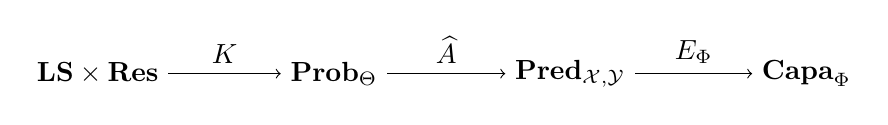
\begin{tikzpicture}[node distance=3.0cm] 
    \node (SR) at (0,0) {$\LS \times \Res$}; 
    \node (Prob) at (3,0) {$\Probt$}; 
    \node (Pred) at (6,0) {$\Pred$}; 
    \node (Val) at (9,0) {$\Capa$}; 
    \draw[->] (SR) -- node[above] {$K$} (Prob); 
    \draw[->] (Prob) -- node[above] {$\widehat{A}$} (Pred); 
    \draw[->] (Pred) -- node[above] {$E_\Phi$} (Val); 
    \end{tikzpicture}
\end{definition}

Expected capability is not an ad hoc numerical operation — it is the unique functor obtained by composing: training (producing distributions), prediction (mapping distributions to kernels), evaluation (mapping kernels to ordered values).

This perspective reveals why expected capability satisfies the monotonicity axiom:
the poset structure of $\Res$ and $\Capa$ ensure that every morphism
\[
(S,R)\to (S,R')
\]
induces
\[
m_\Phi(S,R)\preceq _\Phi m_\Phi(S,R').
\]
Emergence is therefore encoded categorically as structural changes in this functor.

\subsection{Emergence}

Not all learning systems can have certain abilities emerge. We cannot train an MLP with 2 layer, expecting to achieve a $m_\Phi>0.99$ on a parity capability with length 64. That's not how machine learning works, so naturally we will need tools to answer the question "when is a capability $\Phi$ representable by a learning system $S\in \mathcal S $?"

\begin{definition}
    Let $m_\Phi:\mathcal S\times \mathbf R \to \mathcal V$ be the capability function associated with capability type $\Phi$. Define the trivial capability floor by
    \[
    c_{\min} := \inf_{R\in \mathbf R} m_\Phi(S,R)
    \]
    Then $\Phi$ is \textit{representable} by $S$ if and only if
    \[
    \sup_R m_\Phi(S,R)>c_\min
    \]
    Equivalently, $\Phi$ is \textit{representable} by $S$ if and only if there exists a $R^*\in \mathbf R$ and an open neighborhood $N(R^*)$ such that $m_\Phi(S,R)>c_\min$ for all $R\in N(R^*)$
\end{definition}

\begin{definition}{Representability Practically}{}
    Let $m_\Phi:\mathcal S\times \mathbf R \to \mathcal V$ be the capability function associated with capability type $\Phi$, and let $\tau_\Phi :\mathcal S \times \mathbf R \to \R$ be a \textit{representability threshold functional}, assigning to each $(S,R)\in \mathcal S \times \mathbf R$ a reference value of capability requried to count as successful. Then, a capability $\Phi$ is said to be \textit{representable} by a learning system $S$ at resources $R$ if
    \[
    m_\Phi(S,R)\ge \tau_\Phi(S,R)
    \]
    The set of all such pairs is the \textit{representability region}
    \[
    \mathbf R_\Phi(S):=\{R\in \mathbf R : m_\Phi(S,R)\ge \tau_\Phi(S,R)\}
    \]
\end{definition}

Representability expresses achievability: it formalizes when a capability type can be realized by a given system under sufficient resources. The threshold $\tau_\Phi$ can be constant, task-dependent, or empirically defined (e.g., human-level accuracy, baseline reward, statistical significance). By treating it as a functional rather than a scalar constant, the definition remains fully general and coordinate-free.

The structure of the representability region $\mathbf R_\Phi(S)$ within the resource base determines where new capabilities appear. Its boundaries correspond to critical surfaces, and its one-dimensional intersections define representability thresholds along chosen resource directions.

\begin{definition}{Representability Threshold Along a Resource Axis}{}
    Let $\psi:\mathbf R \to \R^k$ be a resource chart and $\alpha\in (R^k)^*$ be an efficient direction. The \textit{representability threshold} of capability type $\Phi$ for system $S$ along direction $\alpha$ is
    \[
    \rho_\Phi(S;\alpha):=\inf \{s(R)=\alpha ^\top \psi(R): m_\Phi(S,R)\ge \tau_\Phi(S,R)\}
    \]
    It gives the minimal effective resource scale along $\alpha$ at which $S$ represents capability $\Phi$.
\end{definition}

\subsubsection{Critical Surfaces}

\begin{definition}[Iso Capability]\label{def:iso-capability}
    For any fixed capability value $c\in \R$, define the \textit{iso-capability set}
    \[
    \Sigma_c(S,\Phi):= \{R\in \mathbf R:m_\Phi(S,R)=c\}
    \]
\end{definition}

Level sets of $m_\Phi(S,R)$ describe the geometry of the capability landscape. Points where $\nabla _Rm_\Phi$ changes discontinuously or the topology of $\Sigma_c$ changes define critical surfaces, which mark transitions in representability—the formal analogue of emergent “phase boundaries” in learning behavior.

\subsubsection{Gauge Equivalence}

\begin{definition}{Gauge Equivalence}{}
    Let $\psi,\psi':\mathcal \R \to \R^k$ be resource charts, $\alpha,\alpha' \in (\R^k)^*$ be directions, and let $f,f':\R\to \R$ be smooth, strictly increasing, S-shaped functions. Then, we say that the triples $(\psi,\alpha,f)$ and $(\psi' , \alpha' ,f')$ are \textit{resource-equivalent}, written
    \[
    (\psi,\alpha,f)\sim (\psi',\alpha',f')
    \]
    if and only if there exists an invertible matrix $A\in GL(k)$, a vector $c\in \R^k$, and scalars $a>0$, $b\in \R$ such that:
    \[
    \psi'(R)=A\psi(R)+c,\quad \alpha' =(A^{-1})^\top \alpha ,\quad f'(x)=f(ax+b) 
    \]
\end{definition}

This gauge equivalence tells us how different coordinate choices $\psi$, directions $\alpha$, and nonlinear profiles $f$ can be transformed into each other without changing the model’s behavior.

\section{Axioms of Emergence Theory}

\subsection{Purpose and Structure of the Axiomatic Framework}

We now specify the formal assumptions that define the space of admissible learning systems. These assumptions are divided into two tiers: structural regularity conditions, and the fundamental axioms of emergence

The following framework distinguishes between assumptions, postulates, and axioms. The assumptions ensure the mathematical well-posedness of the objects of the theory. The postulates express geometric regularities as identified by \citet{bronstein2021geometric} that define the admissible class of learning systems. The axioms (A1–A5) state the fundamental behavioral laws of emergence. While these statements are currently presented as independent, future work may investigate their logical dependencies—specifically whether the geometric postulates (G1–G3) can be derived from the emergence axioms, thereby reducing the theory to a minimal, independent core.

This makes it possible for the axioms of our theory to even speak sensibly. But conceptually, we can call only the second layer the “axioms of emergence.” The first layer is just the mathematical substrate. The axioms of the theory will depend on these base assumptions, and that's fine.

\subsection{Axioms of the Physics of Learning}

The theory rests on four axioms that jointly specify the ``physics'' governing 
how learning systems behave under scaling.  
These axioms fall naturally into three conceptual groups:

\begin{itemize}
    \item \textbf{Group I: Existence Axiom} (ensuring capabilities are not vacuous),
    \item \textbf{Group II: Structural Axioms} (continuity and monotonicity of training),
    \item \textbf{Group III: Emergent Universality} (the one-dimensional law).
\end{itemize}

Each group reflects a qualitatively different kind of assumption: logical existence, 
regularity conditions, and empirical universality.  
Together, they define the landscape on which emergence unfolds.

\subsubsection{Group I: Existence of Capability Realization}

Before one can study emergence, one must ensure that the capability in question 
is not logically or mathematically empty.  
This is encoded in a minimal existence axiom.

\begin{axiom}[Axiom of Representability]\label{axi:representability}
For every capability type whose task is realizable in principle, there exists at least one learning system $S\in\mathcal S$ and at least one resource configuration 
$R\in \mathbf R$ such that $\Phi$ is representable at $(S,R)$.
\end{axiom}

This axiom ensures that the capability function $m_\Phi$ is not the trivial constant function.  
It guarantees that the capability is realizable \emph{somewhere} in the joint space 
of learning systems and resources.  
Without this, the remaining axioms would be vacuous: one cannot study emergence if 
there is nothing that can emerge.

If removed, the entire theory could collapse to the degenerate case where every capability has 
zero (or baseline) performance regardless of resources.  
This would make representability and scaling meaningless.

\subsubsection{Group II: Structural Axioms of Learning Dynamics}

The next two axioms encode the structural regularity of 
learning dynamics: monotonicity with respect to resources and 
continuity with respect to both system and resource variations.  
These play the same role as smoothness and order axioms in classical physics.

\begin{axiom}[Capability Monotonicity]\label{axi:capability-monotonicity}
Let $\mathbf R$ be any resource base, and fix a learning system $S=(\mathbf D , P)$. Then, for $R_1,R_2\in \mathbf R$:
\[
R_1 \preceq R_2 \Rightarrow m (S,R_1)\le m(S,R_2)
\]
\end{axiom}

This axiom says: \emph{increasing resources cannot make a model worse, on average}.  
The coupling formulation expresses this as a relation between distributions 
over trained states.  
It does not assume determinism — only that training with more resources yields 
a stochastically better distribution of outcomes.

If removed, capability monotonicity would no longer hold, the geometry of iso-capability surfaces 
could be pathological, and scaling laws would fail.  
This axiom is equivalent to “more training never reduces the expected skill.”

\subsubsection{Group III: Universality and the One-Dimensional Law}

The final axiom captures the empirical phenomenon that, in the regime where 
a capability is representable and sufficiently smooth,  
all multi-dimensional resource tradeoffs collapse onto a single effective axis.

\begin{axiom}[Axiom of Universality]\label{axi:universality}
There exists an equivalence class $[\psi,\alpha,f]$ such that for every learning system 
$S\in\mathcal S$ in a local neighborhood of procedures,
\[
m_\Phi(S,R)\;\approx\; f\!\left(\alpha^\top \psi(R)\right),
\]
where:
\begin{enumerate}
    \item $\psi:\mathbf R\to \mathbb R^k$ is a continuous resource chart of the resource base,
    \item $\alpha\in (\mathbb R^k)^*$ is an efficient direction,
    \item $f:\mathbb R\to\mathbb R$ is a smooth, monotonically increasing scaling function.
\end{enumerate}
\end{axiom}

Although resources are multi-dimensional (data, parameters, compute, optimization steps),  
emergence depends effectively on a single scaling variable  
\[
s(R)=\alpha^\top\psi(R).
\]
Every capability collapses onto a one-dimensional manifold of effective resource.  
The invariance under affine changes of $\psi$ and $\alpha$ expresses that the law is 
about the \emph{collapse itself}, not particular coordinates.

If removed, the theory would be a purely qualitative description of capability geometry.  
There would be no reason to expect predictable scaling curves, 
no effective axes, and no universality across architectures or procedures.  
This axiom encodes the empirical ``scaling collapse'' at the heart of deep learning.

\subsection{Postulates of Geometric Regularity (G1-G3)}

In addition to the above measure-theoretic regularity, we impose three conditions. The following postulates specify the geometric structure that admissible learning systems must satisfy within the domain defined in Chapter 2. They internalize the geometric priors identified by \citet{bronstein2021geometric}) and ensure that the expected capability functional $m_\Phi(S,R)$ is invariant, stable, and hierarchical.

\begin{definition}{Geometric Regularity 1 (G1) — Symmetry}{}
There exists $G$ acting measurably on $\Omega$ and $C$ such that for every $g\in G$,
\[
(g\cdot x )(\omega)=g_C (x(g_\Omega^{-1}(\omega)),\quad x\in \mathcal X, \ \omega \in \Omega, \ g\in G
\]
Each predictor $\Pi_\theta :\mathcal X \to \mathcal P (\mathcal Y)$ is $G$-equivariant:
\[
\Pi_\theta(g\cdot x)=g\cdot \Pi_\theta(x),
\]
and the capability functional respects this symmetry:
\[
m_\Phi(S,R)=m_\Phi(g\cdot S, R) \quad \forall g\in G.
\]
\end{definition}

This postulate says that learning systems live in a geometric universe: every admissible system $S\in \mathcal S$ carries an invariance structure $G$ describing transformations that preserve meaning. In GDL, this corresponds to equivariance under domain symmetries. In our theory, it ensures that capability depends on intrinsic structure, not on arbitrary parameterizations.

\begin{definition}{Geometric Regularity 2 (G2) — Stability to Deformations}{}
Let $d_\mathcal D$ be a metric on the space of domains and $d_\mathcal X$ a norm on signals. Then for all $S,S'\in \mathcal S$ and fixed $R\in \mathbf R$,
\[
| m_\Phi(S,R) - m_\Phi(S',R) | \le C_\Phi\, d_\mathcal{D}(D,D') + C'_\Phi\, d_\mathcal{X}(x,x').
\]

This is a Lipschitz continuity condition of the capability functional with respect to deformations of the domain or signal. It ensures that small geometric perturbations—changes in data geometry or learned representation—produce only small changes in capability. It gives mathematical expression to robustness and continuity of learning.

This postulate sits naturally on top B7 (continuity of composition).

\end{definition}

\begin{definition}{Geometric Regularity 3 (G3) — Scale Separation}{}
There exists a filtration of the resource manifold
\[
\mathbf R_1\subset \mathbf R_2 \subset \cdots \subset \mathbf R_J =\mathbf R
\]
and corresponding projections
\[
P_j:\mathcal X \to \mathcal X_j
\]
such that capability decomposes hierarchically:
\[
m_\Phi(S,R_J)=F_\Phi(P_J,\dots,P_1),\quad m_\Phi(S,R_{j+1})\ge m_\Phi(S,R_j)
\]
and the incremental gains decrease with $j$.
\end{definition}

This expresses the hierarchical, multi-scale composition principle. It ties the resource space $\mathbf R$ to emergent capability: increasing resources extends the receptive field of the system, but returns diminish with scale.
It mirrors GDL’s “scale separation” prior and links directly to A4–A5 axioms on monotonicity and scaling laws.

The geometric regularity conditions extend the basic structural assumptions by incorporating the invariance and stability principles that \citet{bronstein2021geometric} identified as necessary for expressive architectures. The next section introduces the axioms of emergence (A1–A5), which specify how capability behaves within this structured domain.

\section{Canonical Instantiations and Experiments}

The preceding chapters developed a fully abstract framework for learning systems: topological spaces of data domains and procedures, a resource base equipped with a resource chart, a stochastic training kernel, predictor kernels, and a seed-averaged capability functional $m_\Phi(S,R)$ that serves as an order parameter for emergence. This structure is intentionally architecture-agnostic; it is meant to describe any learning system compatible with the axioms, rather than any particular model or implementation.

A mathematical theory of an empirical domain, however, only acquires content once its objects can be realized. In probability theory, random variables become meaningful through concrete constructions on measurable spaces; in statistical mechanics, spin systems are instantiated on lattices with explicit Hamiltonians; in Geometric Deep Learning, abstract equivariant maps are realized as graph and grid neural networks. In the same spirit, the present framework must be linked to actual training pipelines before its axioms can be interpreted as more than formal constraints.

This chapter instantiates the abstract framework in concrete learning systems. Each section defines a closed learning world, instantiates all objects of the theory, and formulates empirical questions and falsifiable predictions.

\subsection{MLPs}
\subsection{CNNs}

\label{subsec:instantiation-framework}

\section{Theoretical Consequences}

\subsection{The Scaling Law}

\subsubsection{Continuity of Capability}

\begin{lemma}[Boundedness and continuity of the instance capability]\label{lem:Mphi-cont}
The instance capability
\[
M_\Phi(\theta)
  = \E_{(x,y)\sim\mu}
    \E_{y'\sim\Pi_\theta(\cdot|x)}[\,S(y',y)\,]
\]
is bounded and continuous on $\Theta$.
\end{lemma}
\begin{proof}
Boundedness follows immediately from the Definition of Utility \ref{def:learning-utility}: Since 
\[
|S(y',y)|\le \|S\|_\infty
\]
for all \((y',y)\), we have
\[
|M_\Phi(\theta)|
  = \left|\E_{(x,y)\sim\mu}\,\E_{y'\sim\Pi_\theta(\cdot\mid x)}
         [S(y',y)]\right|
  \le \|S\|_\infty.
\]

For continuity, let $\theta_n\to\theta$. By Axiom \ref{axi:kernel-continuity},
\[
\Pi_{\theta_n}(\cdot\mid x)\Rightarrow \Pi_\theta(\cdot\mid x)
\quad\text{for each }x.
\]
Since $S$ is bounded and continuous in its first argument,
\[
\E_{y'\sim\Pi_{\theta_n}(\cdot\mid x)}[S(y',y)]
   \longrightarrow
\E_{y'\sim\Pi_\theta(\cdot\mid x)}[S(y',y)]
\quad\text{for each }(x,y).
\]

To pass the limit through the outer $\mu$-integral, recall from Definition of State Capability \ref{def:state-capability} that
\[
M_\Phi(\theta)
  = \int_{\mathcal X\times\mathcal Y}
      \left(
         \int_{\mathcal Y} S(y',y)\,
         \Pi_\theta(dy'\mid x)
      \right)\mu(dx,dy).
\]

For each $n$, define
\[
f_n(x,y)
  :=
  \int_{\mathcal Y} S(y',y)\,
     \Pi_{\theta_n}(dy'\mid x),
\quad
f(x,y)
  :=
  \int_{\mathcal Y} S(y',y)\,
     \Pi_{\theta}(dy'\mid x).
\]
Then
\[
M_\Phi(\theta_n)=\int_{\mathcal X\times\mathcal Y} f_n(x,y)\,d\mu(x,y),
\quad
M_\Phi(\theta)=\int_{\mathcal X\times\mathcal Y} f(x,y)\,d\mu(x,y).
\]

We have $f_n(x,y)\to f(x,y)$ for every $(x,y)$, and by boundedness of $S$,
\[
|f_n(x,y)|\le \|S\|_\infty
\quad\text{for all }n,(x,y).
\]
Since $f_n(x,y)\to f(x,y)$ pointwise, the dominated
convergence theorem (Appendix \ref{app:dct} yields
\[
\int_{\mathcal X\times\mathcal Y} f_n(x,y)\,d\mu(x,y)
   \;\longrightarrow\;
\int_{\mathcal X\times\mathcal Y} f(x,y)\,d\mu(x,y).
\]
Thus $M_\Phi(\theta_n)\to M_\Phi(\theta)$.
\end{proof}


\begin{lemma}[Local continuity of the expected capability]\label{lem:mphi-cont}
The expected capability
\[
m_\Phi(S,R)
  = \int_\Theta M_\Phi(\theta)\,dK(S,R)(\theta)
\]
is continuous on procedure-local neighborhoods.
\end{lemma}

\begin{proof}
\emph{continuity of $m_\Phi$ via Portmanteau.}
Fix a procedure-local neighborhood $U\subseteq\mathcal S\times\mathbf R$.
Let $(S_n,R_n)\to(S,R)$ with $(S_n,R_n),(S,R)\in U$.
By Axiom \ref{axi:kernel-continuity},
\[
K(S_n,R_n)\ \Rightarrow\ K(S,R)\qquad\text{in }(\Prob(\Theta),\tau_{\rm weak}).
\]
Since $M_\Phi$ is bounded and continuous by Lemma \ref{lem:Mphi-cont}, the Portmanteau theorem yields
\[
\int_\Theta M_\Phi(\theta)\,dK(S_n,R_n)(\theta)\ \longrightarrow\
\int_\Theta M_\Phi(\theta)\,dK(S,R)(\theta).
\]
That is, $m_\Phi(S_n,R_n)\to m_\Phi(S,R)$. Thus $m_\Phi$ is sequentially continuous on $U$. Because the procedure-local topology on $\mathcal S\times\mathbf R$ is first-countable (hence sequential), sequential continuity implies continuity. Therefore $m_\Phi$ is continuous on $U$.

\end{proof}

In summary:

\begin{theorem}[Continuity of Capability]\label{thm:capability-cont}
Under Basic Regularities \textnormal{(B1)--(B9)},
the capability functions $M_\Phi$ and $m_\Phi$
are bounded and continuous on their respective domains.
\end{theorem}

\subsubsection{Capability Monotonicity}

\begin{theorem}[Capability Monotonicity]\label{thm:capability-monotonicity}
Fix a capability type $\Phi$ and a system $S\in\mathcal S$.
If $R_1\preceq R_2$ in the resource base $(\mathbf R,\oplus,0,\preceq,\tau_{\mathbf R})$, then
\[
m_\Phi(S,R_1)\;\le\; m_\Phi(S,R_2)
\]
\end{theorem}

\begin{proof}
By the Axiom of Kernel Monotonicity \ref{axi:kernel-monotonicity}, the training kernel $K$ is monotone compatible with the resource order:
$R_1\preceq R_2$ implies the existence of a coupling $\gamma$ of $K(S,R_1)$ and $K(S,R_2)$ such that
$M_\Phi(\theta_1)\le M_\Phi(\theta_2)$ for $\gamma$-a.e.\ $(\theta_1,\theta_2)$.
Taking expectations under $\gamma$ gives
\[
\mathbb E_{\theta_1\sim K(S,R_1)}[M_\Phi(\theta_1)]
\;\le\;
\mathbb E_{\theta_2\sim K(S,R_2)}[M_\Phi(\theta_2)],
\]
hence $m_\Phi(S,R_1)\le m_\Phi(S,R_2)$.
\end{proof}

\begin{corollary}[Upward-closed superlevel sets; frontier = level set; codimension-1]\label{cor:upward-frontier}
Fix $\Phi$ and $S$. For any $c\in\mathbb R$, the superlevel set
\[
U_c(S,\Phi):=\{R\in\mathbf R:\; m_\Phi(S,R)\ge c\}
\]
is upward-closed: if $R\in U_c$ and $R\preceq R'$, then $R'\in U_c$.
If, in addition, $m_\Phi(S,\cdot)$ is continuous on a neighborhood of $U_c$, then
\[
\Sigma_c(S,\Phi):=\{R:\; m_\Phi(S,R)=c\}=\partial U_c.
\]
If furthermore $m_\Phi(S,\cdot)$ is $C^1$ near $\Sigma_c$ and $c$ is a regular value
($\nabla_R m_\Phi(S,R)\neq 0$ on $\Sigma_c$ in any Euclidean chart of a resource chart),
then $\Sigma_c(S,\Phi)$ is a codimension-$1$ submanifold (hypersurface) of the resource chart.
\end{corollary}

\begin{proof}
Upward-closedness: let $R\in U_c$ and $R\preceq R'$. By Theorem~\ref{thm:capability-monotonicity},
\[
m_\Phi(S,R')\ge m_\Phi(S,R)\ge c,
\]
hence $R'\in U_c$.

Frontier = level set: continuity of $m_\Phi(S,\cdot)$ implies
$U_c=\{m_\Phi\ge c\}$ is closed (preimage of $[c,\infty)$); therefore its boundary equals
$\{m_\Phi=c\}=\Sigma_c$.

Codimension-1: in any Euclidean chart provided by the resource chart,
if $m_\Phi(S,\cdot)$ is $C^1$ and $c$ is a regular value, the regular level set theorem yields
that $\Sigma_c$ is a $(k-1)$-dimensional embedded submanifold, i.e.\ codimension $1$.
\end{proof}

\subsubsection{Existence of an Scaling Functional}

\begin{lemma}[Universality implies existence of an scaling functional]\label{lem:effective-direction}
Suppose Axiom~\ref{axi:universality} (Universality) holds on a procedure-local neighborhood
of $(S,\Phi)$. That is, there exists a triple $[\psi,\alpha,f]$ such that
\[
m_\Phi(S,R)
\;=\;
f\!\left(\frac{\alpha^\top \psi(R)-s^*(S)}{w(S)}\right)
\]
for all $R$ in that neighborhood, and this representation is stable under
resource-equivalence. Then there exists an equivalence class of nonzero
directions $[\alpha]\subset (\R^k)^*$ such that, after quotienting by
resource-equivalence, the iso-capability sets are locally hyperplanes
\[
\{\,R\in\mathbf R:\ \alpha^\top \psi(R)=\text{\rm const.}\,\}
\]
in the resource coordinates $\psi(R)$. Equivalently, in this neighborhood the
capability depends only on the single scalar
\[
s(R) \;=\; \alpha^\top \psi(R),
\]
up to admissible affine reparameterizations of $s$.
\end{lemma}

\begin{proof}
Fix a procedure-local neighborhood $U\subseteq\mathcal S\times\mathbf R$ of
$(S,\Phi)$ on which the Axiom of Universality~\ref{axi:universality} holds with some triple
$[\psi,\alpha,f]$. For the moment, fix the state $S$ and consider the induced
neighborhood
\[
U_S \;:=\; \{\,R\in\mathbf R : (S,R)\in U\,\}.
\]

\medskip
\noindent\textbf{Step 1: Resource-equivalence as a level-set relation.}
On $U_S$, recall the definition of resource equivalence (Definition \ref{def:cap-equiv}):
\[
R \sim R'
\quad\Longleftrightarrow\quad
m_\Phi(S,R) = m_\Phi(S,R').
\]
By definition, iso-capability (Definition \ref{def:iso-capability} sets are precisely the equivalence classes of
$\sim$.

By Universality \ref{axi:universality}, there exist scalars $s^*(S)\in\R$ and $w(S)>0$ and a universal profile $f:\R\to\R$ such that
\[
m_\Phi(S,R)
\;=\;
f\!\left(\frac{\alpha^\top \psi(R)-s^*(S)}{w(S)}\right)
\quad\text{for all }R\in U_S.
\]
Assume $f$ is strictly monotone on the relevant range (as part of the
universality axiom). Then for any $R,R'\in U_S$,
\[
\begin{aligned}
m_\Phi(S,R) = m_\Phi(S,R')
&\quad\Longleftrightarrow\quad
\frac{\alpha^\top \psi(R)-s^*(S)}{w(S)}
=
\frac{\alpha^\top \psi(R')-s^*(S)}{w(S)}\\
&\quad\Longleftrightarrow\quad
\alpha^\top \psi(R)=\alpha^\top \psi(R').
\end{aligned}
\]

Thus the equivalence classes of $\sim$ are exactly the level sets of the scalar
\[
s(R) \;:=\; \alpha^\top \psi(R).
\]

\medskip
\noindent\textbf{Step 2: Iso-capability sets as hyperplanes in resource coordinates.}
Let $z=\psi(R)\in\R^k$ denote the resource coordinates. For any constant
$c\in\R$, the corresponding iso-capability set at level

 \[
 c_0 :=
f\left(\frac{c-s^*(S)}{w(S)}\right)
 \]

is
\[
\begin{aligned}
\{\,R\in U_S : m_\Phi(S,R)=c_0\,\}&
=
\{\,R\in U_S : s(R)=c\,\}\\
&=
\{\,R\in U_S : \alpha^\top \psi(R)=c\,\}.
\end{aligned}
\]
In the coordinate space $\psi(U_S)\subseteq\R^k$, this is the intersection of
$\psi(U_S)$ with the affine hyperplane
\[
H_c \;:=\; \{\,z\in\R^k : \alpha^\top z = c\,\}.
\]
Since $\alpha\neq 0$ (otherwise $m_\Phi$ would be constant in $R$ on $U_S$ and
the universality representation would be degenerate), each $H_c$ is a
codimension-one hyperplane in $\R^k$.

Thus, after quotienting $U_S$ by the equivalence relation $\sim$, the
iso-capability classes are locally represented by hyperplanes
$\{R : \alpha^\top \psi(R)=\text{const.}\}$ in the resource coordinates.

\medskip
\noindent\textbf{Step 3: Scaling Functional up to affine reparameterization.}
The scalar
\[
s(R) = \alpha^\top \psi(R)
\]
is defined only up to affine reparameterizations. Indeed, replacing $s$ by
\[
\tilde{s}(R)
  := \frac{s(R)-s^*(S)}{w(S)}
\]
and correspondingly composing $f$ with an affine change of variables does not
change $m_\Phi(S,R)$. Likewise, replacing $\alpha$ by any nonzero scalar
multiple $\lambda\alpha$ and defining
\[
\tilde{f}(u) := f(u/\lambda)
\]
leads to an equivalent representation of the same capability function. Thus the
scaling functional is determined only up to nonzero scalar multiples; we
denote this equivalence class by $[\alpha]\subset (\R^k)^*$.

In summary, universality on $U$ implies the existence of a (projective) class
of nonzero directions $[\alpha]$ such that:
\begin{enumerate}
    \item iso-capability sets coincide with level sets of $s(R)=\alpha^\top\psi(R)$;
    \item these level sets are (local) hyperplanes in the coordinate space; and
    \item $m_\Phi$ depends on $R$ only through $s(R)$, up to affine
          reparameterization of $s$.
\end{enumerate}
This is exactly the claimed existence of an scaling functional.
\end{proof}


\begin{lemma}[Well-defined scaling curve]\label{lem:scaling-curve}
Let $S$ be fixed and let $\alpha$ be an scaling functional as in Lemma \ref{lem:effective-direction}.
Define the scalar
\[
s(R):=\alpha^\top\psi(R).
\]
Then the map
\[
f_S:\ s\mapsto m_\Phi(S,R)\qquad\text{for any }R\text{ with }s(R)=s
\]
is well-defined, monotone, and continuous.
Consequently,
\[
m_\Phi(S,R)=f_S\bigl(\alpha^\top\psi(R)\bigr)
\]
up to admissible affine reparameterizations of $s$.
\end{lemma}

\begin{proof}
\emph{Well-definedness.}
By Lemma \ref{lem:effective-direction},
\[
R\sim R'
\quad\Longleftrightarrow\quad
s(R)=s(R').
\]
Thus, if $s(R)=s(R')$, then $m_\Phi(S,R)=m_\Phi(S,R')$, so $f_S$ is well-defined.

\medskip
\noindent\emph{Monotonicity.}
By Universality \ref{axi:universality}, there exists a strictly monotone profile $f$ such that
\[
m_\Phi(S,R)=f\!\left(\frac{s(R)-s^*(S)}{w(S)}\right)
\]
on a procedure-local neighborhood.
Since $s(R)$ is an affine functional of $\psi(R)$ and $f$ is strictly monotone, the resulting $f_S$ is monotone in~$s$.

\medskip
\noindent\emph{Continuity.}
By Theorem \ref{thm:capability-cont}, $R\mapsto m_\Phi(S,R)$ is continuous. Since
\[
R\mapsto s(R)=\alpha^\top\psi(R)
\]
is continuous, the quotient map $R\mapsto s(R)$ is continuous, and therefore the induced single-variable function $f_S$ is continuous.

This establishes the representation
\[
m_\Phi(S,R)=f_S(s(R))
=f_S(\alpha^\top\psi(R)),
\]
up to the admissible affine reparameterizations allowed in Universality \ref{axi:universality}. 
\end{proof}

\subsubsection{The Scaling Law}

\begin{theorem}[Scaling law]\label{thm:scaling-law}
Let $(S,\Phi)$ be an admissible learning system. Then there exists a procedure-local
scaling map $f_S$ such that
\[
m_\Phi(S,R)
  = f_S\bigl(\alpha^\top \psi(R)\bigr)
\]
for all $R$ in a procedure-local neighborhood of $S$, up to admissible affine reparameterizations of the scalar
\[
s(R)=\alpha^\top\psi(R).
\]
\end{theorem}

\begin{proof}
Fix an admissible learning system $(S,\Phi)$. By Universality \ref{axi:universality}, there exists a procedure-local
neighborhood $U\subseteq\mathcal S\times\mathbf R$ of $(S,\Phi)$ and a representation triple $[\psi,\alpha,f]$ such that
\[
m_\Phi(S,R)
  = f\!\left(\frac{\alpha^\top\psi(R)-s^*(S)}{w(S)}\right)
\]
for all $R$ with $(S,R)\in U$, and this representation is stable under gauge equivalence.

By Lemma \ref{lem:effective-direction}, there exists an scaling functional $\alpha\neq 0$ such that, after quotienting by capability equivalence at $S$,
the iso-capability sets
\[
\{\,R\in\mathbf R : m_\Phi(S,R)=\text{\rm const.}\,\}
\]
are locally given by hyperplanes
\[
\{\,R\in\mathbf R : \alpha^\top\psi(R)=\text{\rm const.}\,\}
\]
in the resource coordinates $\psi(R)$.
Equivalently, in this neighborhood the capability depends on $R$ only through
the scalar
\[
s(R) := \alpha^\top\psi(R),
\]
up to admissible affine reparameterizations of $s$.

Now fix $S$ and consider the induced neighborhood
\[
U_S := \{\,R\in\mathbf R : (S,R)\in U\,\}.
\]
Define $f_S$ on the image
\[
I_S := s(U_S)\subseteq\R
\]
by
\[
f_S(s) \coloneqq m_\Phi(S,R)
\quad\text{for any }R\in U_S\text{ with }s(R)=s.
\]
By Lemma~\ref{lem:scaling-curve}, this definition is well-defined (i.e.
independent of the choice of $R$ with $s(R)=s$), and the resulting map $f_S$
is monotone and continuous in $s$. Moreover, Lemma~\ref{lem:scaling-curve}
shows that
\[
m_\Phi(S,R) = f_S\bigl(s(R)\bigr)
             = f_S\bigl(\alpha^\top\psi(R)\bigr)
\]
for all $R\in U_S$, up to the admissible affine reparameterizations of $s$
allowed by Universality~\ref{axi:universality} (i.e.\ rescalings and shifts of $s$ absorbed
into a corresponding redefinition of $f_S$).

This is exactly the claimed scaling law for the fixed system $S$.
Since $S\in\mathcal S$ was arbitrary, the conclusion holds for each admissible
learning system.
\end{proof}

\subsection{Criticality and Phase Geometry}

\subsection{Backpropagation as a Derived Principle}
https://chatgpt.com/g/g-p-68a088c3c5b081918671bb266c308f51-ai-research/c/690ab849-f1b0-8331-9904-ba89cf358a53

\subsection{Universality and Resource Equivalence}

\section{Experimentation—Trying My Absolute Best To Break My Theory}

When you axiomatize an empirical domain like modern AI, you’re not declaring truths, but instead you’re proposing tight, testable axioms that compress messy behavior into a few operational claims. Each axiom turns vague talk of “emergence” into specific predictions about a continuous order parameter that should rise along an effective resource axis, align across different ways of spending resources, stay stable within a defined training regime, and be immune to arbitrary reparameterization. Making these axioms falsifiable maximizes information gain. A confirming result means the lens has real predictive bite; a failure tells you exactly where the world refuses the simplification—which knob (data, parameters, steps, context length, precision, data quality) breaks curve collapse, which metric creates mirages, which procedure shift moves the onset or sharpness. In this hybrid program, experiments don’t just “validate” theory; they carve its domain of validity, turning broad conjectures into precise, procedure-local laws and revealing the minimal assumptions under which capability transitions actually behave like scaling phenomena worth proving later.

\clearpage

\appendix
\section{Mathematical Appendix}
\label{app:mathdefs}

\subsection{Probability- and Measure Theory}

\subsubsection{Measurable Structure}


\begin{definition}[$\sigma$-Algebra]\label{app:sigma-algebra}
Let $X$ be a nonempty set.  
A \textit{$\sigma$-algebra} $\mathcal F$ on $X$ is a collection of subsets of $X$ satisfying:
\begin{enumerate}
    \item $X \in \mathcal F$,
    \item if $A \in \mathcal F$, then $A^c = X \setminus A \in \mathcal F$,
    \item if $\{A_i\}_{i=1}^\infty \subseteq \mathcal F$, then $\bigcup_{i=1}^\infty A_i \in \mathcal F$.
\end{enumerate}
Elements of $\mathcal F$ are called \textit{measurable sets}.  
The $\sigma$-algebra encodes the subsets of $X$ to which a measure may consistently assign sizes or probabilities.  
The smallest $\sigma$-algebra containing a family $\mathcal G \subseteq 2^X$ is called the \textit{$\sigma$-algebra generated by} $\mathcal G$, written $\sigma(\mathcal G)$.
\end{definition}

\begin{definition}[Measurable Space]\label{app:measurable-space}
A \textit{measurable space} is a pair $(X,\mathcal F)$, where $X$ is a set and $\mathcal F$ is a $\sigma$-algebra on $X$.  
It provides the structural notion of which subsets of $X$ are admissible for measure and integration.
\end{definition}

\begin{definition}[Measure]\label{app:measure}
Let $(X,\mathcal F)$ be a measurable space.  
A \textit{measure} is a function $\mu : \mathcal F \to [0,\infty]$ such that:
\begin{enumerate}
    \item $\mu(\emptyset) = 0$,
    \item (Countable additivity) if $\{A_i\}_{i=1}^\infty$ are disjoint in $\mathcal F$, then
    \[
    \mu\!\left(\bigcup_{i=1}^\infty A_i\right) = \sum_{i=1}^\infty \mu(A_i).
    \]
\end{enumerate}
A measure assigns "size" or "mass" to measurable sets in a consistent way.  
If $\mu(X) = 1$, we call $\mu$ a \textit{probability measure} and $(X,\mathcal F,\mu)$ a \textit{probability space}.
\end{definition}

\begin{definition}[Measurable Map]\label{app:measurable-map}
Let $(X,\mathcal F_X)$ and $(Y,\mathcal F_Y)$ be measurable spaces.  
A function $f : X \to Y$ is \textit{measurable} if
\[
f^{-1}(A) \in \mathcal F_X \quad \text{for all } A \in \mathcal F_Y.
\]
That is, the preimage of every measurable set in $Y$ is measurable in $X$.  
This ensures that measures defined on $X$ and $Y$ interact coherently under $f$, enabling the construction of \textit{pushforward measures}
\[
f_\# \mu(A) = \mu(f^{-1}(A))
\]
and the definition of integrals $\int f\, d\mu$.
\end{definition}

The concept of measurability provides the bridge between topology and probability.  
It ensures that mappings between domains—such as signals $x : \Omega \to C$ in the main text—preserve the structure necessary to define probabilities and expectations.  
Without measurability, integrals like $\mathbb E[x]$ or probability measures on images $x(\Omega)$ would be undefined.

In the main theory, every space that carries probabilistic structure (data domains, parameter spaces, value spaces) is equipped with a Borel $\sigma$-algebra generated by its topology. Measurable maps—signals, kernels, and predictors—are functions that respect these structures.

\subsubsection{Borel Structure}
\label{app:borel}

\begin{definition}[Borel $\sigma$-algebra]
Let $(X,\tau)$ be a topological space.  
The \emph{Borel $\sigma$-algebra} on $X$, denoted $\mathscr B(X)$, is the smallest $\sigma$-algebra containing all open sets of $X$.  
The elements of $\mathscr B(X)$ are called \emph{Borel sets}.
\end{definition}

The Borel $\sigma$-algebra is the minimal collection of subsets of $X$ to which one can assign probabilities or measures while remaining consistent with the topology.  
It allows us to integrate and talk about probabilities without leaving the structure of the underlying space.  
In our framework, $\Theta$, $\mathcal S$, and $\mathbf R$ all carry their natural topologies, and we use their corresponding Borel $\sigma$-algebras to define measurable maps such as the training kernel
\[
K:(\mathcal S\times\mathbf R,\B(\mathcal S\times\mathbf R))
  \longrightarrow (\Prob(\Theta),\B(\Prob(\Theta))) ,
\]
where:
\[
\B(\Prob(\Theta)):=\text{Borel}(\tau_{\mathrm{weak}})
\]

If $\mathcal S$ and $\mathbf R$ are Polish, then
$\B(\mathcal S\times\mathbf R)=\B(\mathcal S)\times\B(\mathbf R)$.

\begin{definition}[Borel measurable function]
Let $(X,\mathscr A)$ and $(Y,\mathscr B)$ be measurable spaces.  
A map $f:X\to Y$ is \emph{(Borel) measurable} if for every $B\in\mathscr B$,
\[
f^{-1}(B)\in \mathscr A.
\]
\end{definition}

Measurability ensures that the pre-image of any event we can \textit{measure} in $Y$ remains measurable in $X$.  
It is the minimal condition required for integrals like $\int f\,d\mu$ to make sense.  

A measurable function $f:X\to\mathbb R$ is \textit{bounded} if $\sup_{x\in X}|f(x)|<\infty$.  
Boundedness guarantees that integrals against probability measures are finite, a property used throughout the theory for quantities such as $M_\Phi(\theta)$ and $m_\Phi(S,R)$.

\textbf{Relevance in this theory.}
\begin{itemize}
    \item The capability function $M_\Phi:\Theta\to\mathbb R$ must be Borel measurable so that expectations $\int M_\Phi\,dK(S,R)$ are well-defined.
    \item The kernel $K$ itself is measurable in the sense that $(S,R)\mapsto K(S,R)(A)$ is measurable for every Borel set $A\subseteq\Theta$.
    \item Boundedness of $M_\Phi$ ensures that all integrals and expectations are finite and continuous under weak convergence.
\end{itemize}

\subsubsection{Probability Spaces and Measures}
\label{app:probability-spaces-measures}

\begin{definition}{Measure space}{}
A \emph{measure space} is a triple $(X,\mathscr A,\mu)$ where:
\begin{itemize}
    \item $X$ is a set (the underlying space),
    \item $\mathscr A$ is a $\sigma$-algebra of subsets of $X$ (the measurable sets),
    \item $\mu:\mathscr A\to[0,\infty]$ is a measure satisfying:
    \begin{enumerate}
        \item $\mu(\emptyset)=0$,
        \item For any countable family of disjoint sets $(A_i)_{i=1}^\infty\subseteq\mathscr A$,
        \[
        \mu\!\left(\bigcup_{i=1}^\infty A_i\right)=\sum_{i=1}^\infty\mu(A_i).
        \]
    \end{enumerate}
\end{itemize}
\end{definition}

A measure space is a rigorous way of assigning "size" or "volume" to sets, even in cases where standard geometry fails. For instance, on $\mathbb R^d$, Lebesgue measure generalizes the notion of length, area, and volume to very irregular sets.

\begin{definition}{Probability space}{}
A \emph{probability space} is a measure space $(X,\mathscr F,\mathbb P)$ where $\mathbb P(X)=1$.
\end{definition}

A probability space describes all possible outcomes (the sample space $X$), the events we can talk about (the $\sigma$-algebra $\mathscr F$), and how likely each event is (the measure $\mathbb P$).  

In context, every learning configuration $(S,R)$ induces a probability space:
\[
(\Theta,\mathscr B(\Theta), K(S,R)),
\]
where $K(S,R)$ acts as a probability measure over parameter states $\theta$. This makes $(\Theta,\mathscr B(\Theta),K(S,R))$ a valid probability space on which we can define and integrate measurable functions like $M_\Phi(\theta)$.


\begin{definition}{Borel probability measure}{}
Let $(X,\tau)$ be a topological space and let $\mathscr B(X)$ denote its Borel $\sigma$-algebra. A \emph{Borel probability measure} on $X$ is a measure $\mu:\mathscr B(X)\to[0,1]$ satisfying $\mu(X)=1$.

We denote by $\Prob(X)$ the set of all Borel probability measures on $X$.When $X$ is Polish, $(\Prob(X),\tau_{\mathrm{weak}})$ is also Polish (by Prokhorov’s theorem), making it the natural codomain for Markov kernels.
\end{definition}

A Borel probability measure assigns probabilities to all Borel subsets of a topological space.
It is the most natural way to extend the idea of “probability distributions” to general spaces:
instead of describing probability by densities or histograms,
a Borel measure simply says which subsets of $X$ have what probability mass.

All probability measures appearing in this theory—those produced by the training kernel $K(S,R)$, the predictors $\Pi_\theta$, and the data distribution $\mu$—are Borel probability measures.
This guarantees:
\begin{itemize}
    \item Compatibility with the topological structure of $\mathcal S$, $\mathbf R$, and $\Theta$ (Regularities B1–B2 and B7).
    \item Applicability of the Portmanteau theorem and weak topology on $\Prob(\Theta)$.
    \item Existence of integrals such as
          \[
          m_\Phi(S,R)
            = \int_\Theta M_\Phi(\theta)\,dK(S,R)(\theta),
          \]
          which are Lebesgue integrals with respect to a Borel probability measure.
\end{itemize}

\begin{definition}[Pushforward measure]
If $f:X\to Y$ is measurable and $\mu$ is a measure on $X$,  
the \emph{pushforward measure} $f_\#\mu$ on $Y$ is defined by
\[
f_\#\mu(B)=\mu(f^{-1}(B)),\qquad B\in\mathscr B(Y).
\]
\end{definition}

Given a probability space $(X,\mathscr A,\mu)$ and an integrable function $f:X\to\mathbb R$,  
the expectation is defined as
\[
\E_\mu[f] := \int_X f\,d\mu.
\]
This is the mathematical backbone of all expressions like  
$m_\Phi(S,R)=\E_{\theta\sim K(S,R)}[M_\Phi(\theta)]$.

\subsubsection{Markov Kernels and Weak Continuity}
\label{app:markov-kernel}

\begin{definition}{Markov kernel}{}
Let $(X,\mathscr A)$ and $(Y,\mathscr B)$ be measurable spaces.  
A function $K:X\times\mathscr B\to[0,1]$ is a \emph{Markov kernel} if:
\begin{enumerate}
    \item For each $A\in\mathscr B$, the map $x\mapsto K(x,A)$ is $\mathscr A$-measurable.
    \item For each $x\in X$, the map $A\mapsto K(x,A)$ is a probability measure on $(Y,\mathscr B)$.
\end{enumerate}
\end{definition}

It associates to each point $x\in X$ a probability measure on $(Y,\mathcal B)$ such that, for every measurable set $B\in \mathcal B$, the map $x\mapsto\kappa (B,x)$ is measurable with respect to the $\sigma$-algebra $\mathcal A$.

If a deterministic function gives you one point, a Markov kernel gives you a whole distribution. We can see kernels as a stochastic function: A Markov kernel is a stochastic map: instead of sending $x$ to a single point of $Y$, it sends $x$ to a probability distribution on $(Y,\B(Y))$ in a measurable way.

In practice, kernels let us say “the output is random, but in a controlled, measurable way," which is exactly why we use it in defining the training kernel. Without the kernel being measurable, the composed quantity
\[
(S,R)\mapsto \int_\Theta M_\Phi(\theta)\,dK(S,R)(\theta)
\]
would not be guaranteed measurable; this property is crucial in Lemma~\ref{lem:wellposed-cont}.

\begin{definition}{Weak continuity}{}
Let $\Theta$ be a Polish space with Borel $\sigma$-algebra $\mathscr B(\Theta)$.
A Markov kernel $K:(\mathcal S\times\mathbf R)\to \Prob(\Theta)$ is said to be
\emph{weakly continuous} if, for every sequence $(S_n,R_n)\to(S,R)$ in $\mathcal S\times\mathbf R$,
\[
K(S_n,R_n)\Rightarrow K(S,R)
\quad\text{in }(\Prob(\Theta),\tau_{\text{weak}}),
\]
i.e.\ for all bounded continuous $f:\Theta\to\mathbb R$,
\[
\int_\Theta f(\theta)\,dK(S_n,R_n)(\theta)
   \longrightarrow
\int_\Theta f(\theta)\,dK(S,R)(\theta).
\]
\end{definition}

Weak continuity ensures that small perturbations in the system or resource parameters produce only small changes (in the weak sense) in the resulting distribution of trained parameters. This is the formal notion behind the idea that "training behaves continuously" with respect to $(S,R)$.

This property connects the geometry of the learning domain $\mathcal S\times\mathbf R$ with the probabilistic space $\Prob(\Theta)$. It is the assumption used in Lemma~\ref{lem:wellposed-cont} to guarantee the continuity of $m_\Phi(S,R)$ via the Portmanteau theorem.

\noindent\textbf{Remark.}
Because $\mathcal S\times\mathbf R$ and $\Prob(\Theta)$ are Polish, sequential weak continuity is equivalent to topological continuity with respect to $\tau_{\mathrm{weak}}$.

\subsubsection{Weak Convergence and Topologies}
\label{app:weak-topology}
Reference: Billingsley (1968), Villani (2009).

Let $\Theta$ be a Polish space with Borel $\sigma$-algebra $\mathscr B(\Theta)$.
Denote by $\Prob(\Theta)$ the set of Borel probability measures on $\Theta$.

\begin{definition}{Weak convergence}{}
A sequence $(\mu_n)\subseteq \Prob(\Theta)$ is said to \emph{converge weakly} to $\mu\in\Prob(\Theta)$, written
$\mu_n\Rightarrow\mu$, if
\[
\int_\Theta f(\theta)\,d\mu_n(\theta)\longrightarrow
\int_\Theta f(\theta)\,d\mu(\theta)
\quad\text{for every bounded continuous }f:\Theta\to\mathbb R.
\]
\end{definition}

\begin{definition}{Weak Topology}{}
    The \textit{weak topology} is the coarsest topology such that, for every bounded continuous $f:\Theta\to \R$, the map
    \[
    \mu \longmapsto \int_\Theta f(\theta) \ d\mu(\theta)
    \]
    is continuous.
\end{definition}

So a sequence of distributions $(\mu_n)$ converges weakly to $\mu$ if every continuous measurement of the system sees the same averages in the limit. That is, even if individual samples from $\mu_n$ fluctuate wildly, their aggregate expectations on smooth observables stabilize. In context, $f(\theta)=M_\Phi(\theta)$ is one such observable, measuring capability. The weak topology ensures that small changes in $(S,R)$, hence in the distribution $K(S,R)$, can produce small changes in expected capabilities $m_\Phi(S,R)$.

\subsubsection{Portmanteau Theorem}
\label{app:portmanteau}

\begin{theorem}{Portmanteau}{}
For probability measures $\mu_n,\mu\in\Prob(\Theta)$ on a metric space $\Theta$, the following are equivalent:
\begin{enumerate}
    \item $\mu_n\Rightarrow\mu$.
    \item For all bounded continuous $f:\Theta\to\mathbb R$,
    \[
    \int f\,d\mu_n \to \int f\,d\mu.
    \]
    \item For every closed set $F\subseteq\Theta$,
    \[
    \limsup_{n\to\infty}\mu_n(F)\le\mu(F).
    \]
    \item For every open set $G\subseteq\Theta$,
    \[
    \liminf_{n\to\infty}\mu_n(G)\ge\mu(G).
    \]
\end{enumerate}
\end{theorem}

Weak convergence formalizes the idea that distributions are close when they give similar expectations to all smooth observables. It governs the continuity of integrals when the measures vary (contrast with the Dominated Convergence Theorem, which governs limits when the functions vary).

\begin{corollary}{Continuity of integrals under weak convergence}{}
If $\mu_n \Rightarrow \mu$ and $f$ is bounded and continuous, then $\int f\,d\mu_n \to \int f\,d\mu$.
\end{corollary}

This is important since for the training kernel
\[
K:(\mathcal S\times\mathbf R,\tau_\mathcal S\times\tau_\mathbf R)
   \longrightarrow (\Prob(\Theta),\tau_{\text{weak}}),
\]
and any bounded continuous capability function $M_\Phi:\Theta\to\mathbb R$,
the Portmanteau theorem implies
\[
K(S_n,R_n)\Rightarrow K(S,R)
\Longrightarrow
\int M_\Phi\,dK(S_n,R_n)\to \int M_\Phi\,dK(S,R),
\]
which yields the local continuity of
$m_\Phi(S,R)=\E_{\theta\sim K(S,R)}[M_\Phi(\theta)]$
established in Lemma 1 of the main text.

\subsubsection{Lebesgue Integration}
\label{app:lebesgue}

\begin{definition}[Lebesgue integral]
Let $(X,\mathscr A,\mu)$ be a measure space and $f:X\to[0,\infty]$ a measurable function.
The \emph{Lebesgue integral} of $f$ with respect to $\mu$ is defined as
\[
\int_X f\,d\mu = \sup\left\{
   \int_X s\,d\mu \; :\;
   s \text{ is a simple function with } 0\le s\le f
\right\},
\]
where a simple function is a finite linear combination
$s(x)=\sum_{i=1}^n a_i\mathbf 1_{A_i}(x)$ with $A_i\in\mathscr A$ and $a_i\ge0$.
For general (possibly signed) measurable $f$, we define
\[
\int f\,d\mu = \int f^+\,d\mu - \int f^-\,d\mu,
\]
where $f^+=\max(f,0)$ and $f^-=\max(-f,0)$.
\end{definition}

Lebesgue integration measures the "weighted area" under $f$ by first cutting the \emph{range} of $f$ into levels rather than partitioning the \emph{domain} as in Riemann integration. It is designed to handle discontinuities, limits, and arbitrary measurable domains robustly.

Riemann integration only works when the domain is an interval and $f$ is nearly continuous everywhere.  
Lebesgue integration, on the other hand, can integrate over arbitrary measurable sets and with respect to arbitrary measures. In our case, we integrate over $(\Theta,\mathscr B(\Theta),K(S,R))$, where $K(S,R)$ is a probability measure that may not have a density or any geometric structure. Thus, the integral
\[
\int_\Theta M_\Phi(\theta)\,dK(S,R)(\theta)\eqqcolon m_\Phi(S,R)
\]
is necessarily a \emph{Lebesgue integral.}

Known properties:
\begin{itemize}
    \item \textbf{Linearity:} $\int (a f + b g)\,d\mu = a\int f\,d\mu + b\int g\,d\mu$.
    \item \textbf{Monotone convergence:} If $0\le f_n\uparrow f$, then $\int f_n\,d\mu\uparrow\int f\,d\mu$.
    \item \textbf{Dominated convergence:} If $|f_n|\le g\in L^1(\mu)$ and $f_n\to f$ pointwise, then $\int f_n\,d\mu\to\int f\,d\mu$.
    \item \textbf{Absolute integrability:} If $\int |f|\,d\mu<\infty$, we write $f\in L^1(\mu)$.
\end{itemize}

Relevance to this theory:
\begin{itemize}
    \item All expectations, such as $\E_{\theta\sim K(S,R)}[M_\Phi(\theta)]$, are Lebesgue integrals on the probability space $(\Theta,\mathscr B(\Theta),K(S,R))$.
    \item Lebesgue integration allows us to handle continuous, discontinuous, or even infinite-dimensional parameter spaces uniformly.
    \item Theorems like Dominated Convergence (Appendix~A.x+2) guarantee that taking limits and integrating over $\Theta$ commute—crucial for proving continuity and scaling-law results.
\end{itemize}

For example, if $\Theta=\mathbb R^d$ and $K(S,R)$ has a density $p_{S,R}(\theta)$,  
then the Lebesgue integral reduces to the familiar expression
\[
m_\Phi(S,R)=\int_{\mathbb R^d} M_\Phi(\theta)\,p_{S,R}(\theta)\,d\theta,
\]
which is the Riemann integral weighted by the density, but the general Lebesgue form remains valid even when $p_{S,R}$ does not exist.

\subsubsection{Dominated Convergence Theorem}
\label{app:dct}

\begin{theorem}{Dominated Convergence}{}
Let $(X,\mathscr A,\mu)$ be a measure space and let $(f_n)_{n\in\mathbb N}$ be a sequence of measurable functions 
$f_n:X\to\mathbb R$ such that $f_n(x)\to f(x)$ for $\mu$-almost every $x\in X$.
Assume there exists an integrable function $g\in L^1(\mu)$ satisfying
\[
|f_n(x)|\le g(x) \quad \text{for all } n\in\mathbb N,\ \text{for $\mu$-a.e. }x\in X.
\]
Then $f$ is integrable and
\[
\lim_{n\to\infty}\int_X f_n\,d\mu=\int_X f\,d\mu.
\]
\end{theorem}

The theorem allows one to interchange limits and integrals when the functions themselves vary, provided that all are \textit{dominated} by a common integrable envelope $g$.
It ensures continuity of the map $f\mapsto \int f\,d\mu$ under pointwise convergence with uniform integrability.
In our setting this is used internally, e.g.\ when defining
\[
M_\Phi(\theta)=\E_{(x,y)\sim\mu}\E_{y'\sim \Pi_\theta(\cdot|x)}[U(y',y)],
\]
to justify passing limits through expectations as the inner functions vary.

\subsection{Topology and Functional Analysis}

\subsubsection{Topological Vector and Banach Spaces}
\label{app:tvs}

\subsubsection{Hausdorff and Polish Spaces}
\label{app:hausdorff-polish}

\begin{definition}[Hausdorff space]
A topological space $(X,\tau)$ is \emph{Hausdorff} if for any two distinct points $x_1,x_2\in X$, there exist open sets $U,V\in\tau$ such that
\[
x_1\in U,\quad x_2\in V,\quad U\cap V=\emptyset.
\]
\end{definition}

The Hausdorff property ensures that points can be separated by neighborhoods. In a Hausdorff space, limits of sequences (if they exist) are unique. This property is the minimal separation requirement for doing analysis. Without it, the notion of continuity or convergence becomes ambiguous.

The Hausdorff condition is built into most of our spaces—$\mathcal S$, $\mathbf R$, and $\Theta$—so that
limits of parameter sequences $\theta_n\to\theta$ or procedure sequences $(S_n,R_n)\to(S,R)$ are well-defined. It ensures the continuity statements in Lemma~\ref{lem:Mphi-cont} and Lemma~\ref{lem:mphi-cont} have an unambiguous sense of “approaching a unique limit.”


\begin{definition}[Polish space]
A \emph{Polish space} is a topological space that is separable and completely metrizable;
that is, there exists a metric $d$ on $X$ such that:
\begin{enumerate}
    \item $(X,d)$ is complete: every Cauchy sequence converges in $X$;
    \item $(X,d)$ is separable: there exists a countable dense subset $D\subseteq X$.
\end{enumerate}
\end{definition}

Polish spaces strike the perfect balance between richness and manageability: they are large enough to include infinite-dimensional and function spaces, but structured enough for all standard convergence and measure-theoretic results to hold. They are the canonical stage for probability theory and functional analysis.

Basic Regularity (B7) asserts that $\Theta$ is Polish. This guarantees:
\begin{itemize}
    \item Weak convergence of measures (used in B8 and Lemma~\ref{lem:mphi-cont}) is well-defined and metrizable.
    \item Compactness/tightness arguments can be applied when studying scaling limits.
    \item $\Prob(\Theta)$ is itself Polish, allowing kernels
          $K:(\mathcal S\times\mathbf R)\to\Prob(\Theta)$
          to be treated with standard continuity theorems.
\end{itemize}

In short, the “Polish” assumption ensures that our learning domain behaves like a well-structured infinite-dimensional manifold where probability, continuity, and convergence all coexist harmoniously.


\begin{definition}[Sequential continuity]
Let $(X,\tau_X)$ and $(Y,\tau_Y)$ be topological spaces and let $f:X\to Y$. The map $f$ is said to be \emph{sequentially continuous} at $x\in X$ if, for every sequence $(x_n)\subseteq X$ with $x_n\to x$ in $\tau_X$, we have
\[
f(x_n)\to f(x)\quad\text{in }\tau_Y.
\]
It is \emph{sequentially continuous} on $X$ if it is sequentially continuous at every $x\in X$.
\end{definition}

In general, sequential continuity is a weaker condition than topological continuity: it only checks the preservation of convergence for sequences, while full continuity requires the preimage of every open set in $Y$ to be open in $X$. However, in first-countable spaces—those whose topology can be captured by sequences—the two notions coincide.

\begin{proposition}[Equivalence in metric and Polish spaces]
If $X$ is a metric (hence Hausdorff and first-countable) space and $Y$ is any topological space, then a map $f:X\to Y$ is continuous if and only if it is sequentially continuous. In particular, this holds for all Polish spaces.
\end{proposition}

\begin{proof}[Proof sketch]
If $f$ is continuous, it is sequentially continuous by definition. Conversely, suppose $f$ is sequentially continuous.
In metric spaces, a set $U\subseteq X$ is open iff for every $x\in U$ there exists $\varepsilon>0$ such that $B_\varepsilon(x)\subseteq U$, which is equivalent to saying that no sequence from $X\setminus U$ can converge to $x$.
Sequential continuity ensures that the image of any convergent sequence preserves this property, so $f^{-1}(V)$ is open whenever $V$ is open in $Y$. Hence $f$ is continuous.
\end{proof}

In metric (and therefore Polish) spaces, sequences capture all possible modes of convergence. So verifying continuity via sequences is not merely sufficient—it is \textit{equivalent}. This equivalence is why proofs on Polish spaces often conclude with the line: \emph{“sequential continuity implies continuity.”}

In Lemma~\ref{lem:mphi-cont}, we showed that
\[
m_\Phi(S_n,R_n)\to m_\Phi(S,R)
\]
whenever $(S_n,R_n)\to(S,R)$ and $K(S_n,R_n)\Rightarrow K(S,R)$. This gives \emph{sequential} continuity of $m_\Phi$.
Because $(\mathcal S\times\mathbf R,\tau_\mathcal S\times\tau_\mathbf R)$ is Polish by Regularities (B1)--(B2),
sequential continuity immediately implies topological continuity. Thus the assumption that our learning spaces are Polish is what allows the proof to close cleanly.

The equivalence between sequential and topological continuity is more than a technicality—it expresses the deep regularity of the spaces your theory operates on. Because your learning domains are Polish, you can safely reason about convergence entirely in terms of sequences (as we did in Lemma~\ref{lem:mphi-cont}), without invoking nets or filters. This makes the theory operationally elegant and aligns it with the way machine-learning processes actually behave in practice: training procedures, parameter updates, and data limits are all naturally sequential.

\subsubsection{Function-Space Topologies}
\label{app:function-space-topologies}

\begin{definition}{Pointwise convergence topology}{}
Let $Y^X$ denote the set of all functions $f:X\to Y$, where $(Y,\tau_Y)$ is a topological space.
The \emph{pointwise convergence topology} on $Y^X$ is the coarsest topology such that,
for every $x\in X$, the evaluation map
\[
\mathrm{ev}_x : f \mapsto f(x)
\]
is continuous.
A sequence $(f_n)$ converges to $f$ pointwise if $f_n(x)\to f(x)$ for each $x\in X$.
\end{definition}

\begin{definition}{Compact-open topology}{}
Let $(X,\tau_X)$ be a topological space and $(Y,\tau_Y)$ a metric space.
The \emph{compact-open topology} on $C(X,Y)$, the space of continuous maps $X\to Y$, is generated by subbasic sets of the form
\[
W(K,U)=\{\,f\in C(X,Y):f(K)\subseteq U\,\},
\]
where $K\subseteq X$ is compact and $U\subseteq Y$ is open.
\end{definition}

Many objects in the theory are function-valued:
\begin{itemize}
    \item the predictor $\Pi_\theta:\mathcal X\to\Prob(\mathcal Y)$,
    \item the training map $K:(\mathcal S\times\mathbf R)\to\Prob(\Theta)$,
    \item the capability function $M_\Phi:\Theta\to\R$.
\end{itemize}
Each lives naturally in a function space. By equipping these spaces with appropriate function topologies, we can speak rigorously of continuity and convergence of mappings between them.

Specifically:
\begin{itemize}
    \item The continuity of $\theta\mapsto\Pi_\theta$ in (B4) is continuity
          in a weak function-space topology on $\Prob(\mathcal Y)$.
    \item The continuity of $(S,R)\mapsto K(S,R)$ in (B8) is continuity
          in the function-space topology on $\Prob(\Theta)$ induced by the weak topology.
    \item Lemma~\ref{lem:Mphi-cont} and Lemma~\ref{lem:mphi-cont}
          rely on these topologies to interpret weak convergence and ensure that
          expectations vary smoothly under parameter and resource perturbations.
\end{itemize}

Thus, function-space topologies give the geometric foundation for treating learning systems as continuous transformations between probability spaces.

\subsubsection{Wasserstein Metric and Optimal Transport}
\label{app:w-metric}

Distributions are "close" if we can rearrange one into the other with little effort.

Formally, let $(X,d)$ be a metric space. Let $\mathcal P _p(X)$ be the set of Borel probability measures $\mu$ on $X$ with finite $p$-th moment:
\[
    \int_X d(x,x_0)^p\mu(dx)<\infty
\]
for some arbitrary reference point $x_0\in X$.

For $\mu, \nu\in \mathcal P _p(X)$, a \textit{coupling} is a joint distribution $\gamma$ on $X\times X$ with marginals $\mu$ and $\nu$:

\[
    \gamma(A\times X)=\mu (A),\quad \gamma(X\times B)=\nu(B)
\]

for all measurable $A,B\subseteq X$

Then, the \textit{Wasserstein-}$p$ distance is:
\[
    W_p(\mu,\nu)=\left(\inf_{\gamma\in \Gamma(\mu,\nu)}\int_{X\times X} d(x,y)^p d\gamma(x,y)\right)^{1/p}
\]
where $\Gamma(\mu, \nu)$ is the set of all couplings.

So 
\subsubsection{Kantorovich–Rubinstein Duality}
\label{app:kantorovich–rubinstein-duality}

\subsubsection{Product and Compact-Open Topologies}
\label{app:open-compact-topologies}

\subsubsection{First-countability and sequential continuity}

\subsubsection{The Dual Space}

\subsubsection{The General Linear Group}

\subsubsection{Linear Functionals}

\subsubsection{Affine Hyperplanes}

\subsubsection{Affine reparameterization and gauge freedom}

\subsubsection{Continuity of Functionals and Measurable Maps}
\label{app:continuity-of-functionals}

\subsection{Algebraic and Structural Foundations}

\subsubsection{Equivalence Relations and Classes}
\label{app:equivalence-relations}

\subsubsection{Quotient Structures}
\label{app:equivalence-relations}

\subsubsection{Partial Orders and Resource Topologies}
\label{app:partial-order}

\subsubsection{Monoids and Homomorphisms}
\label{app:monoids}

\subsubsection{Symmetry and Group Actions}
\label{app:equivalence-relations}

\subsection{Category Theory}

\subsubsection{Categories}
\label{app:categories}

\subsubsection{Discrete Categories}
\label{app:discrete-categories}

\subsubsection{Monoidal Categories}
\label{app:monoidal-categories}

\subsubsection{Poset Categories (Thin Categories)}
\label{app:poset-categories}

\subsubsection{Monads}
\label{app:monads}

\subsubsection{Kleisli Categories}
\label{app:kleisli-categories}

\subsection{Statistics and Learning Theory}

\subsubsection{Order Parameters and Phase Transitions}
\label{app:order-parameter}

\subsubsection{Lipschitzness}
\label{app:lipschitzness}

% References
\newpage
\bibliographystyle{abbrvnat}
\bibliography{references}

\end{document}
